%--------------------------------------------------------------------------------------%--------------------------------------------------------------------------------------
%
%  Global settings, dont change it! (excapt additional \usepackage commands)
%  Always use PDFLatex!
%
%--------------------------------------------------------------------------------------%--------------------------------------------------------------------------------------
\documentclass[a4paper, 12pt, oneside, BCOR1cm,toc=chapterentrywithdots]{scrbook}

\usepackage{graphicx}           % use for pdfLatex
\usepackage{makeidx} % f\"{u}r Benutzung des Befehls \printindex
\usepackage[colorlinks=false]{hyperref}
\usepackage{cleveref}
\usepackage{tocbibind}
\usepackage{subfigure}
\usepackage[nohyperlinks]{acronym}
\usepackage{longtable}
\usepackage{array}   % ragged-right p{} columns in the wide tables
\usepackage{tikz}
\usetikzlibrary{positioning,fit,arrows.meta,calc}
\usepackage{xcolor}
\usepackage[section]{placeins} % forces a float barrier at every \section,
                                % so a table/figure can never queue past the
                                % section that introduces it

\hypersetup{%
bookmarksnumbered=true, hyperindex=true,
%
%Im Acrobat Reader Subtitel 1. Ebene anzeigen
bookmarksopen=true, bookmarksopenlevel=1,
%
pdfborder=0 0 0 % Keine Box um die Links!
}

% --------------------------------------------------------------
% Force Tables and List to be added in Table of Content
% --------------------------------------------------------------

\renewcommand*{\tableofcontents}{%
  	\begingroup
  	\tocsection
  	\tocfile{\contentsname}{toc}
  	\endgroup
}
\renewcommand*{\listoffigures}{%
  	\begingroup
  	\tocsection
  	\tocfile{\listfigurename}{lof}
  	\endgroup
}
\renewcommand{\listoftables}{
	\begingroup
	\tocsection
	\tocfile{\listtablename}{lot}
	\endgroup
}
\begin{document}

%--------------------------------------------------------------------------------------%--------------------------------------------------------------------------------------
%
%  Here starts the userspace !
%
%--------------------------------------------------------------------------------------%--------------------------------------------------------------------------------------

%--------titlepage
\begin{titlepage}

{
    \begin{center}
        \raisebox{-1ex}{
\includegraphics[scale=1.5]{TU_Chemnitz_positiv_gruen.pdf}}\\
    \end{center}
    \vspace{0.5cm}
}

\begin{center}

\LARGE{\textbf{Integrating Open Large Language Models into the Jupyter
Notebook Reproducibility Pipeline}}\\
\vspace{1cm}


\Large{\textbf{Master Thesis}}\\
\vspace{1cm}
Submitted in Fulfilment of the\\
Requirements for the Academic Degree\\
M.Sc. Web Engineering\\
\vspace{0.5cm}
Dept. of Computer Science\\
Chair of Computer Engineering
\end{center}

\vfill

\noindent
Submitted by: Erisa Zaimi\\
Student ID:\\
Date: [Submission Date]

\bigskip

\noindent
Supervising tutor: Dr. Sheeba Samuel

\vspace{1cm}
\end{titlepage}

%---------------------------------------------------------
% Abstract
%---------------------------------------------------------

\addchap*{Abstract}
Jupyter notebooks are widely used to share computational research, but a
large share of published notebooks fail to re-execute in a different
environment. The FAIR Jupyter project has studied this problem at scale and
built a pipeline that containerises each repository before execution to
remove many such failures; even so, this pipeline only detects and logs the
dependency-related failures that remain -- it does not explain or repair
them. This thesis adds a repair layer that attaches at exactly that point.

The working dataset is a residual set of 214 dependency-related failures
recorded by the Docker-based pipeline, of which 200 fall inside a pip-only
repair scope defined for this first version of the system. Given a failed
notebook, a deterministic classifier decides its subtype and repair
eligibility before any language model is consulted.

An explanation component produces a plain-language, schema-validated
description of the failure for every classified record, independent of
whether it can later be repaired; it has now been run across all 200
repair-scope rows (the 13-row development split and the 187-row evaluation
split), where it produced a schema-valid explanation for 185 of the 187
evaluation records.

A repair component proposes a concrete
fix using an open,
locally-run large language model whose suggestion is grounded in live
metadata from the Python Package Index and validated, field by field,
against that evidence, so that a proposed package name or version is never
invented. A fix-application component applies a validated proposal inside
an environment rebuilt to match the one the notebook originally failed in,
re-executes the whole notebook, and classifies the result as fixed, still
failing, or not meaningfully testable.

All of these components are implemented and covered by 332 automated tests.

Beyond this component-level testing, the complete repair layer was run
once, unattended, over the reserved 187-row evaluation split, using a real
local language model, the live PyPI registry, and a real Docker daemon
throughout. No notebook in this split reached completely successful
re-execution within the two-round repair budget, but this is not the same
as saying no repair worked: 84.9\% of the 73 real repair attempts made
(across both rounds) removed the specific dependency error they targeted,
and every one of the 73 language-model repair responses obtained during
the run produced a schema-valid, PyPI-grounded proposal. The gap between
these two numbers has two main causes. First, the repair agent's static
import-to-distribution mapping only covered enough failing modules to reach
the language model for 73 of 235 repair-agent invocations across both
rounds (31.1\%); the remaining invocations abstained beforehand rather than
guess an unsupported package name. Second, resolving one dependency error
frequently exposed a second, previously hidden one, and the bounded,
two-round repair budget was not always enough to clear all of them within
the same notebook.

A result-logging component joins the classification, explanation, and
repair records these components already produce into one persistent record
per repair attempt, stored in a SQLite benchmark table, and an RDF mapping
re-expresses that record and links it to the existing FAIR Jupyter knowledge
graph. Both were checked directly against real, pilot-scale data: the
mapping produces syntactically valid RDF that links correctly to existing
notebook resources. The benchmark table has since been populated at the
scale of the full 187-row evaluation run; enriching the knowledge graph from
that larger run, rather than from the pilot sample, remains future work.

All 214 dependency-error
records were confirmed to share notebook identifiers with the inspected
knowledge-graph source data.

This thesis reports work completed through a full evaluation of the
repair layer over the reserved 187-row evaluation split, including a
Round-1-versus-final comparison drawn from that same run. Full-scale
enrichment of the knowledge graph from this evaluation run, an
explanation-quality user study, and a baseline comparison against a
non-grounded repair agent remain future work and are stated as such, rather
than presented as already measured.


\bigskip
\noindent
\textbf{Keywords: Jupyter notebooks, computational reproducibility, large
language models, retrieval-augmented generation, dependency repair}

%---------------------------------------------------------
% Table of Contents, List of figures, List of Tables
%---------------------------------------------------------

\tableofcontents
\listoffigures
\listoftables

%---------------------------------------------------------
% List of Abbreviations
%---------------------------------------------------------
\twocolumn
\addchap{List of Abbreviations}
\begin{acronym}[PROV-O]
 \acro{API}{Application Programming Interface}
 \acro{APR}{Automated Program Repair}
 \acro{FAIR}{Findable, Accessible, Interoperable, Reusable}
 \acro{JSON}{JavaScript Object Notation}
 \acro{KG}{Knowledge Graph}
 \acro{LLM}{Large Language Model}
 \acro{PMC}{PubMed Central}
 \acro{PROV-O}{PROV Ontology}
 \acro{PyPI}{Python Package Index}
 \acro{RAG}{Retrieval-Augmented Generation}
 \acro{RDF}{Resource Description Framework}
 \acro{RML}{RDF Mapping Language}
\end{acronym}

\onecolumn
%---------------------------------------------------------
% Here starts the real work
%---------------------------------------------------------

%---------------------------------------------------------
% Chapter 1: Introduction
%---------------------------------------------------------
\chapter{Introduction}
\label{chap:introduction}

\section{Motivation}
\label{sec:intro-motivation}

Jupyter notebooks combine code, explanatory text, and results in a single
document. This makes them a popular way to share computational research,
especially in data-heavy fields such as biomedicine. A notebook published
alongside a paper is meant to let another researcher see, and re-run, exactly
how a result was produced.

In practice, many published notebooks do not run at all when someone else
tries them. Pimentel et al.~\cite{pimentel2019msr} collected 1.4~million
notebooks from GitHub and attempted to execute a large subset of them: only
24.11\% ran without errors, and only 4.03\% reproduced the results reported by
their original authors. Samuel and Mietchen~\cite{samuel2024gigascience}
found a similar pattern specifically for notebooks accompanying biomedical
publications on PubMed Central, the domain this thesis also builds on. These
numbers show that non-reproducible notebooks are not a rare exception; they
are the common case.

A large share of these failures is caused by dependencies, not by mistakes in
the underlying research logic. A notebook is written against a particular set
of installed Python packages. When it is later run in a different
environment, a package may be missing entirely, or a newer version of a
package may no longer provide the exact function the notebook expects. Both
situations produce an error before the notebook can finish, even though the
scientific code itself may be correct. The resulting error messages are often
short and technical, for example \texttt{ModuleNotFoundError: No module named
'sklearn'}, which is unhelpful to a researcher who is not a software
developer and has no way to know that the fix is to install a package called
\texttt{scikit-learn} rather than \texttt{sklearn}.

\section{The FAIR Jupyter Pipeline and Its Remaining Gap}
\label{sec:intro-gap}

The FAIR Jupyter project has studied this problem at scale. Samuel and
Mietchen~\cite{samuel2024gigascience} built a pipeline that downloads
notebooks referenced by biomedical publications, executes them, and records
whether each notebook ran and, if not, what error occurred. The results were
organised into a queryable knowledge graph~\cite{samuel2024fairkg} so that
patterns in notebook reproducibility could be studied directly. A more recent
extension of the same pipeline~\cite{samuel2025docker} runs every repository
inside its own Docker container before execution. Containerisation removes
many failures that were really about a missing system tool or an
incompatible operating system, rather than about the research code.

Even this containerised pipeline stops at the point of \emph{detecting} a
failure. When a notebook still does not run inside its container, the
pipeline records the exception type and message and moves on. It does not
explain the failure to a human reader, and it does not attempt a fix. Every
notebook whose only problem is a missing or outdated Python package is left
exactly as broken as it was found, even though such problems are, in
principle, straightforward to repair by installing or pinning the right
package version.

This is the gap this thesis addresses: turning a detected, dependency-related
notebook failure into an explained and, where possible, repaired one,
automatically and without a person in the loop for every single notebook.

\section{Contribution of This Thesis}
\label{sec:intro-contribution}

This thesis adds a repair layer on top of the existing Docker-based FAIR
Jupyter pipeline. The pipeline's own contribution ends at logging a failure;
this thesis begins exactly there. Given a notebook execution that failed with
a dependency-related error, the added layer performs five steps:

\begin{enumerate}
  \item \textbf{Classify} the failure: is it really a dependency problem, and
        if so, is it a missing package or an incompatible version?
  \item \textbf{Explain} the failure in plain language, so that a researcher
        without a programming background can understand what went wrong.
  \item \textbf{Propose a repair}, using an open, locally-run large language
        model (LLM) whose suggestion is grounded in live package metadata
        from the Python Package Index (PyPI) rather than left to guess a
        version number from training data.
  \item \textbf{Apply the repair} inside an environment equivalent to the one
        the notebook originally failed in, and re-run the whole notebook from
        the beginning.
  \item \textbf{Record the outcome}: whether the notebook now runs further,
        still fails, or could not be meaningfully tested.
  \end{enumerate}

Grounding the repair suggestion in live PyPI data follows PLLM, the closest
prior system to this one. Bartlett et
al.~\cite{bartlett2025pllm} show that retrieval-augmented generation (RAG)
against live package data measurably improves an LLM's dependency-repair
accuracy compared to letting the model rely on what it happens to remember
from training. This thesis adopts the same principle and applies it inside a
reproducibility pipeline rather than to standalone Python scripts, and adds
an explanation step and a re-execution-based validation step that PLLM does
not have.

\subsection{Objectives}
\label{sec:intro-objectives}

The work is organised around six objectives, first defined in the thesis
vision document and used throughout this text to relate individual
components back to the overall goal.

\begin{table}[h]
  \centering
  \begin{tabular}{|l|p{10.5cm}|}
    \hline
    \textbf{Objective} & \textbf{Description} \\
    \hline
    O1 & Generate a plain-language explanation of a dependency-related failure. \\
    \hline
    O2 & Generate an automated, PyPI-grounded fix suggestion using an open LLM. \\
    \hline
    O3 & Apply the suggested fix and validate it by re-executing the notebook. \\
    \hline
    O4 & Compile a structured, reusable benchmark dataset of failures, fixes, and outcomes. \\
    \hline
    O5 & Integrate the above into the existing FAIR Jupyter pipeline without manual intervention. \\
    \hline
    O6 & Record repair outcomes as RDF triples in the FAIR Jupyter knowledge graph. \\
    \hline
  \end{tabular}
  \caption{Thesis objectives, as defined in the vision document.}
  \label{tab:intro-objectives}
\end{table}

\subsection{Status of This Thesis}
\label{sec:intro-status}

This thesis reports work completed through the result-logging and
knowledge-graph implementation stage of a staged
design-implementation-evaluation plan; \Cref{chap:methodology} explains,
component by component,
how each stage was actually built. As of this stage:

\begin{itemize}
  \item Objectives O1, O2, and O3 are \textbf{implemented and evaluated}: a
        classification and explanation component, a PyPI-grounded repair
        proposal component, and a fix-application-and-re-execution component
        all exist as working, unit-tested code, and have since been run
        together, unattended, over the full 187-row evaluation split
        described in \Cref{chap:problem-dataset}, using a real Ollama model,
        the real PyPI registry, and a real Docker daemon throughout. No
        notebook in this split reached completely successful re-execution
        within the two-round repair budget, but 84.9\% of the 73 real
        repair attempts made across both rounds removed the specific
        dependency error they targeted, and every language-model repair
        response obtained during the run was schema-valid and PyPI-grounded.
        \Cref{chap:validation} reports this evaluation in full.
  \item Objectives O4 and O6 -- the reusable benchmark dataset and
        knowledge-graph enrichment -- are \textbf{implemented and validated
        at pilot scale}: a result-logging component persists one row per
        repair attempt to a SQLite table, and an RDF mapping links each
        logged attempt into the existing FAIR Jupyter knowledge graph. The
        benchmark table has since been populated at the scale of the full
        evaluation run above; enriching the knowledge graph from that larger
        run, rather than from the pilot sample checked in
        \Cref{sec:v-i6}, remains future work.
  \item Objective O5, full pipeline integration, is \textbf{implemented and
        evaluated at full scale}: a single program
        (\texttt{scripts/run\_pipeline.py}) runs all five repair-layer
        components, plus a bounded, max-two-round repair loop, over a given
        slice of the dataset automatically, sharing one run identifier
        across every stage it calls. Beyond the small real pilot that first
        validated this orchestrator (\Cref{sec:v-i7}), it has now driven the
        complete 187-row evaluation run referenced above.
        \Cref{chap:future-work} states exactly what remains.
  \item The evaluation reported in \Cref{chap:validation} is the
        thesis's final evaluation, not only a pilot: it covers the complete
        187-row evaluation split, once, under the same configuration
        throughout. It measures an overall repair success rate together
        with the diagnostic metrics needed to interpret it -- the rate at
        which individual targeted dependency errors were resolved, the rate
        at which the repair agent could reach the language model at all
        given its current package-mapping coverage, and the rate of
        infrastructure faults unrelated to repair quality. \Cref{chap:validation}
        reports each of these in turn, together with what they do and do
        not show about the system.
\end{itemize}

This distinction between what has been implemented and validated, and what
is still planned, is kept explicit throughout this document rather than
blurred for the sake of a stronger-sounding narrative.

\section{Thesis Structure}
\label{sec:intro-structure}

\Cref{chap:related-work} reviews prior work on notebook reproducibility,
automated dependency resolution, and LLM-based program repair, and states
the specific gap this thesis fills. \Cref{chap:problem-dataset} describes the
scale of the reproducibility problem and how the concrete working dataset for
this thesis was obtained. \Cref{chap:architecture} presents the system
architecture: the five components introduced above, their contracts, and the
data they exchange. \Cref{chap:methodology} is the core of the thesis: it
explains, component by component, how each part was actually built, the
decisions made along the way, and where the implementation ended up
differing from the original design. \Cref{chap:validation} reports the
automated test suite, the real-system pilot results obtained during
implementation, and the final evaluation over the full 187-row evaluation
split. \Cref{chap:future-work} separates what is finished from what remains.
\Cref{chap:conclusion} closes the thesis with a summary of the contribution.


%---------------------------------------------------------
% Chapter 2: Background and Related Work
%---------------------------------------------------------
\chapter{Background and Related Work}
\label{chap:related-work}

This chapter reviews the work this thesis builds on and positions its
contribution against it. It covers four areas: measuring notebook
reproducibility, restoring it automatically, using large language models
(LLMs) for dependency resolution and program repair, and the FAIR data
principles that motivate recording repair outcomes in a knowledge graph. The
chapter closes by stating, precisely, the gap none of this prior work closes
on its own.

\section{Reproducibility of Computational Notebooks}
\label{sec:rw-reproducibility}

Computational reproducibility means that a published analysis can be
re-executed by someone else and produce the same result. For a Jupyter
notebook, the weaker and more basic question is whether it can be
\emph{re-executed at all}: does the code still run, independent of whether
the numbers come out identical. This thesis targets that weaker property,
re-executability, as the necessary first step before reproducibility in the
fuller sense can even be discussed.

A large-scale study by Pimentel et al.~\cite{pimentel2019msr} measured
this directly. Out of 1.4~million notebooks collected from GitHub, only 24.11\% of
the notebooks they attempted ran without an error, and only 4.03\% produced
results matching those already stored in the notebook. Samuel and
Mietchen~\cite{samuel2024gigascience} repeated this measurement for
notebooks linked from biomedical publications on PubMed Central and found
the same low reproducibility rate in that domain. This is the dataset this
thesis' own working data is derived from, described in
\Cref{chap:problem-dataset}. Both studies agree on the dominant cause: most
failures are not bugs in the analysis logic, but missing or incompatible
software dependencies.

Detecting these failures is itself useful. Samuel and
K{\"o}nig-Ries~\cite{samuel2020reproducemegit} built ReproduceMeGit, a
visualisation tool that runs the notebooks in a GitHub repository and shows,
for each one, whether it succeeded, crashed, or produced different output
than before. Tools like this make the scale of the problem visible to a
repository owner, but they stop at reporting: they do not explain a failure
in terms a non-programmer can act on, and they do not attempt to fix
anything.

\section{Restoring Executability}
\label{sec:rw-restoring}

A separate line of work tries to go one step further and automatically
restore a broken environment rather than only reporting that it is broken.

\subsection{Static Analysis and Knowledge Graphs}

Wang et al.~\cite{wang2020ase} studied how execution environments could
be reconstructed by analysing a notebook's own code. They followed this
with SnifferDog~\cite{wang2021snifferdog}, a tool that statically
inspects a notebook's imports and matches them against a database of
known package APIs. SnifferDog correctly inferred the required
environment for 92.6\% of the notebooks it was tested on. This result
makes an important point that motivates the present thesis: a notebook
that looks broken is often not broken in its logic at all. It simply
lacks the right dependency information, which can in many cases be
recovered automatically.

A separate family of tools builds this dependency knowledge as an explicit
knowledge graph rather than analysing one notebook at a time. Horton and
Parnin's DockerizeMe~\cite{horton2019dockerizeme} introduced this idea: it encodes
package-to-module mappings from Libraries.io in a graph database and uses it
to infer, and then containerise, the dependencies a Python snippet needs.
Ye et al.'s PyEGo~\cite{ye2022pyego} extended the same idea to a much larger
graph covering third-party packages, the Python interpreter version, and
system libraries together, reporting a 0.4--3.5$\times$ accuracy improvement
over DockerizeMe. Cheng et al. added explicit conflict detection between
transitive dependencies with PyCRE~\cite{cheng2022pycre}, and later refined
the approach with ReadPyE~\cite{cheng2024readpye}, which reached 79.75\%
successful environment reconstruction, the strongest result among the
knowledge-graph approaches reviewed here.

These knowledge-graph approaches share one structural limitation: they can
only recommend a package or version that is represented in their indexed
data. Such a graph must be maintained and updated as new PyPI releases
appear, and a package or release that has not yet been indexed is
unavailable to it until the graph is rebuilt. This limitation motivates
replacing a fixed package-and-version snapshot with a live query against
the package registry itself, which is the design this thesis adopts
(\Cref{chap:architecture}).

\subsection{LLMs for Dependency Resolution}
\label{sec:rw-llm-dep}

Bartlett et al.'s PLLM~\cite{bartlett2025pllm} is the closest prior
system to this thesis and its main point of comparison. PLLM uses an
LLM, retrieval-augmented with live PyPI data, to resolve missing or
incompatible Python dependencies from execution feedback. In their
experiments, an LLM using retrieval-augmented generation (RAG) against
live package data outperformed the strongest knowledge-graph baselines
by a wide margin (+15.97\% fixes over ReadPyE, +21.58\% over PyEGo).
Results were especially strong on notebooks that depend on
machine-learning libraries -- relevant here, since the dataset in
\Cref{chap:problem-dataset} is dominated by exactly such packages
(\texttt{scikit-learn}, \texttt{scipy}, \texttt{tensorflow}). Gao et
al.'s RAG survey~\cite{gao2024ragsurvey} and Tao et al.'s survey of
retrieval-augmented code generation~\cite{tao2025racg} both confirm
that grounding a generative model's output in retrieved, verifiable
facts, rather than the model's own memorised knowledge, is established
practice for exactly this kind of task. This is the basis for Lewis et
al.'s original formulation of retrieval-augmented
generation~\cite{lewis2020rag}.

PLLM differs from this thesis in four ways that matter for the present
design: it operates on standalone Python files, not on notebooks embedded in
a reproducibility pipeline; it uses unbounded multi-round iteration rather
than a fixed number of repair attempts; it produces no human-readable
explanation of the failure; and it does not feed its results into any
knowledge graph. \Cref{sec:rw-gap} returns to each of these points directly.

\subsection{LLM-Based Program Repair and Notebook-Specific Work}
\label{sec:rw-apr}

More broadly, LLM-based automated program repair (APR) is an active
field. Yang et al.'s survey~\cite{yang2025aprsurvey} organises 63
systems published between 2022 and 2025 into four design paradigms:
fine-tuning, prompting, procedural pipelines, and agentic frameworks.
Agentic frameworks, where the model plans and re-plans its own next
action, perform well on complex, multi-file bugs, but at a real cost in
latency and control. That trade-off directly motivates a design
decision explained in \Cref{chap:architecture}: this thesis structures
its repair layer as a fixed, procedural pipeline, not an autonomous
agent, because the target workload is hundreds of independent, mostly
single-dependency notebook failures processed in batch, not a small
number of complex interactive sessions. The same survey also confirms
that retrieval-augmented context improves repair quality across every
paradigm it studied, reinforcing the PyPI-grounding decision from
\Cref{sec:rw-llm-dep}.

Two lines of work are specific to notebooks. Grotov et
al.~\cite{grotov2024untangling} released a dataset of buggy notebooks,
together with a proposed agent design. They followed it
with a full implementation~\cite{grotov2024debug} that observes the
output of each execution attempt, decides what to change, applies it,
and tries again. That second paper establishes a point this thesis
relies on directly: because a notebook keeps state between cells, a
candidate fix can only be judged correct by re-running the
\emph{whole} notebook from the top, not just the cell that originally
failed (\Cref{chap:architecture} adopts this rule for the same reason).
Xia and Zhang's ChatRepair~\cite{xia2024chatrepair} similarly feeds
re-execution feedback back into the next repair attempt, in a
conversational loop, achieving 162 of 337 fixes on a general Python bug
benchmark. The same feedback principle underlies the bounded two-round
repair mode built for this thesis (\Cref{sec:orchestrator}), with one
difference: the budget here is fixed at two rounds rather than left open.
Reyes et
al.'s Byam~\cite{reyes2025byam} and Tang et al.'s
SynFix~\cite{tang2025synfix} both target dependency-aware repair
outside the notebook setting: breaking dependency updates in Java, and
structured cross-file repair, respectively. Both motivate giving the
repair model structured dependency context rather than the bare error
message. This thesis follows that principle in a different form. The
repair prompt carries the classified error (type, message, failing
module, subtype, root-cause hint), the failing cell's source where it
could be recovered, and release evidence retrieved live from PyPI; a
repository's declared requirements are used later, when FixApplicator
reconstructs the execution environment, not as evidence handed to the
repair model (\Cref{sec:m-repair-nodeps}).

On the interactive side, Jupyter AI~\cite{jupyterai2023} lets a user ask an
LLM inside JupyterLab to explain an error or generate a fix. It is a useful
point of contrast: Jupyter AI is designed for one user working on one
notebook at a time and must be triggered manually after every failure. It
has no route into a batch reproducibility pipeline and no connection to the
structured metadata such a pipeline already records. The system built for
this thesis is designed for exactly the opposite situation: no user present,
hundreds of notebooks, and existing structured failure metadata to build on.

Model and prompt choice also draw on this literature. Szalontai et
al.~\cite{szalontai2024codellama} find that a smaller, code-specialised
model can outperform a larger general-purpose one on bug-fixing tasks,
and that prompt design affects repair quality about as much as model
size does. A broader empirical study of LLM-based
APR~\cite{empiricalapr2025} confirms that code-specialised models tend
to lead on Python repair specifically, across more than 600,000
patches. Dinh et al.'s comparison of prompting techniques for code
generation~\cite{dinh2024codeprompteval} informs the structured-output,
few-shot prompt design in \Cref{chap:methodology}. Chain-of-thought
prompting~\cite{wei2022cot} was considered and not adopted: the prompts
request a structured JSON answer with few-shot examples rather than
explicit intermediate reasoning, because the benefit of additional
reasoning prompts for locally deployable models of this size is
uncertain and a second prompt technique would have made the comparison
less controlled. Dinh et al.
in particular find that including a project's declared package list in
the prompt measurably improves dependency-aware generation. The repair
prompt in this thesis applies the same idea to a different, verifiable
source: instead of the project's own package list, it supplies the
candidate releases retrieved live from PyPI for the failing distribution,
so that every version the model can choose is one that is known to exist.

\section{FAIR Principles and Knowledge Graphs}
\label{sec:rw-fair}

The FAIR Jupyter project this thesis extends is itself grounded in the
FAIR principles: that data, and by extension research software, should
be Findable, Accessible, Interoperable, and
Reusable~\cite{wilkinson2016fair}. Barker et al.~\cite{barker2022fair4rs}
extend these principles specifically to research software. They argue
that the Reusable principle for software requires recording the
\emph{provenance} of its execution environment -- not only the code
itself, but the conditions under which it did or did not run. Samuel
and Mietchen's FAIR Jupyter knowledge
graph~\cite{samuel2024fairkg,samuel2024zenodo} already stores exactly
this kind of provenance for the original execution attempts. Recording
a repair attempt in the same graph, using the PROV
ontology~\cite{provenance2013} for the activity/agent/time structure,
extends that existing provenance record to cover repair as well as
detection. This is the basis for objective O6, designed in
\Cref{chap:architecture}, implemented in \Cref{chap:methodology}, and
validated in \Cref{chap:validation} first on pilot data and then over the
complete table of the final evaluation.

\section{Research Gap}
\label{sec:rw-gap}

Taken together, the literature above shows that the individual building
blocks already exist separately. Pipelines exist that detect and record
reproducibility failures at
scale~\cite{samuel2025docker,samuel2024gigascience,samuel2024fairkg}. Tools
exist that infer or restore a missing Python
environment, from static analysis~\cite{wang2021snifferdog} to
knowledge graphs~\cite{horton2019dockerizeme,ye2022pyego,cheng2022pycre,cheng2024readpye}
to live-retrieval LLMs~\cite{bartlett2025pllm}. LLM agents exist that can fix
errors in notebooks specifically, interactively, one session at a
time~\cite{grotov2024untangling,grotov2024debug}. FAIR-aligned provenance
recording exists for the original failures~\cite{samuel2024fairkg}.

Among the systems reviewed for this thesis, none combines all of the
following: (1) an LLM-based repair
layer that runs autonomously, without a user manually triggering each
attempt; (2) inside an existing reproducibility pipeline rather than on
standalone files; (3) with the repair suggestion grounded in live PyPI data
specifically for the pip-based dependency errors that pipeline already
detects; and (4) paired with a plain-language explanation and, eventually,
provenance recorded as RDF linked to the same knowledge graph the pipeline
already produces.

PLLM~\cite{bartlett2025pllm} is the closest system in mechanism, but it is
not pipeline-embedded, does not explain a failure, and does not write to a
knowledge graph. Grotov et al.'s agents~\cite{grotov2024untangling,
grotov2024debug} are the closest for notebooks specifically, but they assume
an interactive session with a live kernel, not an autonomous batch pass over
a pipeline's own residual failures. \Cref{tab:rw-gap} summarises this
positioning against the thesis objectives introduced in
\Cref{chap:introduction}.

\begin{table}[htbp]
  \centering
  \begin{tabular}{|l|p{4.8cm}|p{4.0cm}|}
    \hline
    \textbf{Objective} & \textbf{Gap it fills} & \textbf{Builds on} \\
    \hline
    O1 -- Explanation & None of the reviewed pipelines explains a residual failure in plain language & Grotov~\cite{grotov2024untangling,grotov2024debug}, Jupyter AI~\cite{jupyterai2023} \\
    \hline
    O2 -- PyPI-grounded repair & None of the reviewed systems embeds PyPI-grounded RAG repair inside a reproducibility pipeline & PLLM~\cite{bartlett2025pllm}, Lewis et al.~\cite{lewis2020rag} \\
    \hline
    O3 -- Fix validation & Autonomous, batch re-execution validation is not done by the reviewed notebook agents & ChatRepair~\cite{xia2024chatrepair}, Grotov~\cite{grotov2024debug} \\
    \hline
    O4 -- Benchmark dataset & No reviewed benchmark covers dependency repair on biomedical notebooks & Grotov~\cite{grotov2024untangling}, Pimentel~\cite{pimentel2019msr} \\
    \hline
    O5 -- Pipeline integration & The FAIR Jupyter pipeline stops at logging; no repair layer exists yet & Samuel et al.~\cite{samuel2025docker,samuel2024gigascience,samuel2024fairkg} \\
    \hline
    O6 -- KG enrichment & None of the reviewed systems records repair provenance as FAIR RDF triples & \cite{samuel2024fairkg}, PROV-O~\cite{provenance2013}, \cite{wilkinson2016fair} \\
    \hline
  \end{tabular}
  \caption{Thesis objectives, the gap each one fills, and the prior work it builds on.}
  \label{tab:rw-gap}
\end{table}

This is the gap the remainder of this thesis addresses: a controlled,
package-registry-grounded LLM repair layer for dependency failures in a FAIR
Jupyter notebook pipeline, that also validates its own repairs by
re-executing the notebook, rather than trusting the model's suggestion on
faith.


%---------------------------------------------------------
% Chapter 3: Problem Analysis and Dataset
%---------------------------------------------------------
\chapter{Problem Analysis and Dataset}
\label{chap:problem-dataset}

This chapter answers two questions and keeps them apart. How large is the
reproducibility problem in general, and what exactly does this thesis's
implementation operate on? The first is answered by numbers from the
original, full-scale FAIR Jupyter study. The second is answered by a much
smaller, precisely defined dataset drawn from the newer Docker-based
pipeline. The two are related, because the second is a residual subset of
the same kind of failure, but they are not the same numbers and are never
mixed here.

\section{Scale of the Problem}
\label{sec:pd-l1}

The original FAIR Jupyter study executed every notebook it collected using a
fresh conda environment per repository~\cite{samuel2024gigascience}. The
figures below were recomputed for this thesis from the published database
of that study~\cite{samuel2024zenodo}, using the local snapshot of its
\texttt{executions} table. A notebook counts as executed when its
execution record is neither an environment-installation failure nor a
skipped notebook, and the two exception counts are taken from the recorded
failure reason of each execution:

\begin{itemize}
  \item Total notebooks executed: \textbf{10,389}
  \item \texttt{ModuleNotFoundError}: 5,562 (53.5\%)
  \item \texttt{ImportError}: 1,014 (9.8\%)
  \item Combined dependency-related failures: \textbf{6,576 (63.3\%)}
\end{itemize}

The published article itself reports 10,388 notebooks attempted for
re-execution and 6,588 \texttt{ModuleNotFoundError} and
\texttt{ImportError} exceptions, computed over a different
denominator~\cite{samuel2024gigascience}; the small differences reflect
the counting rule stated above, not a different dataset. In other words,
roughly two out of every three executed notebooks failed for a
dependency-related reason. The missing modules were dominated by
biomedical and machine-learning packages, consistent with the PubMed Central
origin of the dataset: \texttt{anndata} (1258 occurrences),
\texttt{scanpy} (423), \texttt{pandas} (177), \texttt{cemba\_data} (176),
\texttt{tensorflow} (149), \texttt{Bio} (108), and \texttt{fastai} (103) were
the most frequently missing modules in that snapshot.

These numbers exist to establish that dependency failure is a large-scale,
systematic problem, not an edge case worth ignoring. \textbf{They are not the
dataset this thesis's implementation runs on.} They come from the earlier
conda-based run of the pipeline, before the Docker-based extension described
next.

\section{The Working Dataset}
\label{sec:pd-i1}

\subsection{Why the Docker Pipeline, Not the Conda Run}
\label{sec:pd-why-docker}

The newer, containerised pipeline~\cite{samuel2025docker} re-executes
each repository inside its own Docker container. Containerisation
resolves many of the failures counted in \Cref{sec:pd-l1} that were
really caused by a missing system tool or an operating-system mismatch,
not by the notebook's Python dependencies. What is left over after
containerisation -- notebooks that still fail even inside a container
built specifically for them -- is a cleaner, more targeted signal of a
genuine dependency problem. This is why the Docker pipeline, not the
original conda run, was chosen as the integration target. Its residual
failures are exactly the gap this thesis is meant to close. And its
result schema already tags each failure with a pre-computed
\texttt{error\_category}, which removes the need to re-implement
failure detection from scratch.

\subsection{Source and Filtering}
\label{sec:pd-source}

The working dataset is derived from the Docker pipeline's own result
database (\texttt{notebook\_executions} table). Its existing categorisation
routine already maps two exception types into a bucket called
\texttt{DEPENDENCY\_ERROR}: \texttt{ModuleNotFoundError} and
\texttt{ImportError}. These two types were kept, unchanged, as this thesis's
scope, for two reasons: they are exactly what the upstream pipeline already
flags as dependency-related, and, taken together, they cover both a package
being completely absent and a package being present but missing a specific
name the notebook tries to import.

Filtering every row where \texttt{error\_category = 'DEPENDENCY\_ERROR'}
yields \textbf{214} rows: 172 \texttt{ModuleNotFoundError} and 42
\texttt{ImportError}. This extraction and every count in this section is
produced by \texttt{scripts/prepare\_dependency\_dataset.py}, and is written
out as a CSV file plus a machine-readable statistics file so that the
numbers can be independently recomputed.

\subsection{Repair Scope: Why pip-Only}
\label{sec:pd-scope}

Not every one of the 214 rows can be repaired the same way. Version~1 of the
repair layer is restricted, deliberately, to dependency problems that a
single \texttt{pip install} command can fix: installing a missing package,
or pinning a specific version. This scope decision was made for a concrete
reason: it keeps the first version of the system controlled and measurable.
A repair action that also has to reason about system-level packages
(installed with \texttt{apt}, not \texttt{pip}) or about renaming an import
path inside the notebook's own code introduces a second, much larger kind of
decision that this thesis does not attempt to automate yet.

Applying this scope splits the 214 rows into the four subtypes of
\Cref{tab:pd-subtypes}, and those in turn into two groups.

\begin{table}[htbp]
  \centering
  \begin{tabular}{|l|r|p{6.3cm}|}
    \hline
    \textbf{Subtype} & \textbf{Count} & \textbf{Meaning} \\
    \hline
    \texttt{missing\_package} & 179 & The imported module is genuinely absent. \\
    \hline
    \texttt{wrong\_version} & 21 & The module is present, but the notebook imports a name that no longer exists in the installed version. \\
    \hline
    \texttt{system\_library} & 10 & A missing shared object file (e.g.\ \texttt{libxcb.so.1}), installable only with \texttt{apt}, not \texttt{pip}. \\
    \hline
    \texttt{mapping\_unknown} & 4 & An ambiguous local or path-shadowed name (e.g.\ \texttt{utils}) that cannot safely be mapped to a PyPI package. \\
    \hline
  \end{tabular}
  \caption{Dependency-error subtypes across the 214-row working dataset.}
  \label{tab:pd-subtypes}
\end{table}

The 10 \texttt{system\_library} rows are excluded because they need
\texttt{apt}-level installation, which is outside the pip-only scope by
definition. A missing shared library cannot be fixed by any pip
command, however it is phrased. The 4 \texttt{mapping\_unknown} rows are
excluded because their failing name (for example a generic module
called \texttt{utils}) cannot be safely resolved to one specific PyPI
package without guessing. Guessing a package name is exactly the kind
of unfounded suggestion this thesis's PyPI-grounding design
(\Cref{chap:architecture}) is built to avoid. This leaves \textbf{200
usable} rows and \textbf{14 excluded} rows.

\begin{table}[htbp]
  \centering
  \begin{tabular}{|l|r|p{7.5cm}|}
    \hline
    \textbf{Split} & \textbf{Count} & \textbf{Purpose} \\
    \hline
    \texttt{dev} & 13 & Used to design and manually sanity-check the explanation and repair prompts (\Cref{chap:methodology}). \\
    \hline
    \texttt{evaluation} & 187 & Usable rows reserved for the final repair evaluation, reported in \Cref{chap:validation}. \\
    \hline
    \texttt{excluded} & 14 & Within explanation scope; excluded from automated repair (\Cref{sec:pd-explanation-scope}). \\
    \hline
  \end{tabular}
  \caption{Split policy over the 214-row working dataset.}
  \label{tab:pd-splits}
\end{table}

\Cref{tab:pd-splits} shows how the 214 rows divide across the three
resulting splits. The 13-row \texttt{dev} split was used exclusively during
implementation, to design and manually sanity-check the explanation and
repair prompts and to run the small real-system pilots reported in
\Cref{chap:validation}. The
187-row \texttt{evaluation} split was reserved from prompt and
repair-strategy tuning: no prompt, mapping entry, or repair rule was
designed against it. The results reported in \Cref{chap:validation} were
generated using the final frozen implementation described in
\Cref{chap:methodology}.

\subsection{Explanation Scope Is Wider Than Repair Scope}
\label{sec:pd-explanation-scope}

One further decision affects every later chapter and is worth stating
clearly. The pip-only restriction above governs \emph{repair} eligibility
only. It does not restrict \emph{explanation}. All 214 rows, including the
14 excluded ones, stay within the explanation scope defined for objective
O1. Only the 200 usable rows are additionally in scope for the
repair-proposal and fix-application components (objectives O2 and O3). A
researcher whose notebook fails because of a missing system library still
deserves to be told what went wrong, even though the current repair layer
cannot fix that case automatically.

\Cref{fig:pd-scope} shows this scope boundary in one place. Every one of
the 214 records enters classification and stays within the explanation
objective, while only 200 are repair-eligible and feed the rest of the
repair layer.

\begin{figure}[h]
  \centering
  \resizebox{0.92\textwidth}{!}{%
  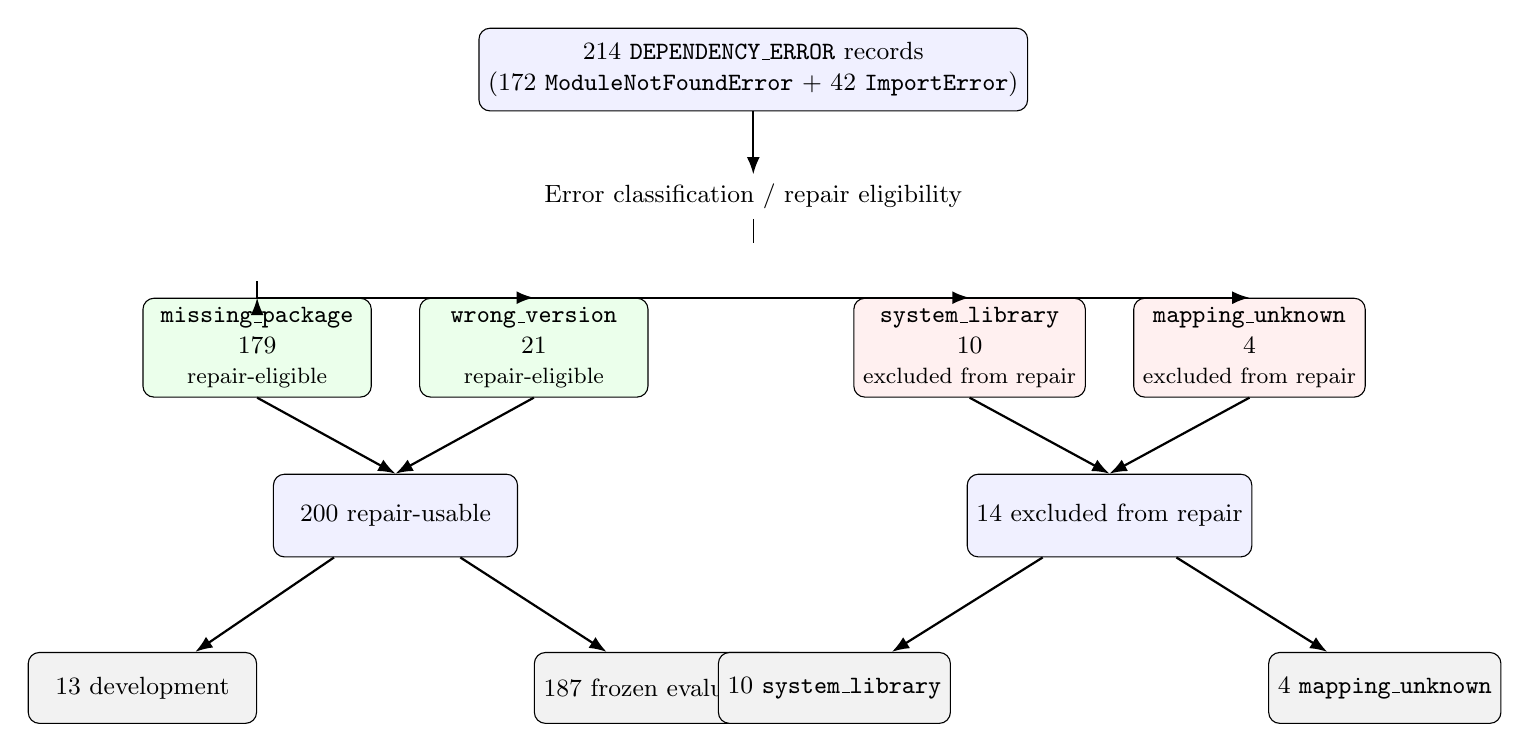
\begin{tikzpicture}[
      font=\small,
      comp/.style={draw, rounded corners, fill=blue!6, minimum width=3.1cm,
                   minimum height=1.05cm, align=center, node distance=8mm},
      elig/.style={draw, rounded corners, fill=green!8, minimum width=2.9cm,
                   minimum height=1.2cm, align=center, node distance=6mm},
      excl/.style={draw, rounded corners, fill=red!6, minimum width=2.9cm,
                   minimum height=1.2cm, align=center, node distance=6mm},
      leaf/.style={draw, rounded corners, fill=gray!10, minimum width=2.9cm,
                   minimum height=0.9cm, align=center, node distance=6mm},
      arr/.style={-{Latex[length=2.2mm]}, thick},
    ]
    % ---------- row of four subtypes ----------
    \node[elig] (c1) {\texttt{missing\_package}\\179\\\footnotesize repair-eligible};
    \node[elig, right=of c1] (c2) {\texttt{wrong\_version}\\21\\\footnotesize repair-eligible};
    \node[excl, right=26mm of c2] (c3) {\texttt{system\_library}\\10\\\footnotesize excluded from repair};
    \node[excl, right=of c3] (c4) {\texttt{mapping\_unknown}\\4\\\footnotesize excluded from repair};

    \coordinate (topmid) at ($(c1)!0.5!(c4)$);
    \node[comp, above=30mm of topmid] (records)
      {214 \texttt{DEPENDENCY\_ERROR} records\\(172 \texttt{ModuleNotFoundError} + 42 \texttt{ImportError})};
    \node[font=\small, below=8mm of records, text width=6cm, align=center] (classify)
      {Error classification / repair eligibility};

    \coordinate (busY) at ($(c1.north)+(0,7mm)$);
    \draw[arr] (records) -- (classify);
    \draw (classify.south) -- (classify.south |- busY);
    \draw (c1.north -| busY) -- (c4.north -| busY);
    \draw[arr] (c1.north -| busY) -- (c1.north);
    \draw[arr] (c2.north -| busY) -- (c2.north);
    \draw[arr] (c3.north -| busY) -- (c3.north);
    \draw[arr] (c4.north -| busY) -- (c4.north);

    % ---------- aggregate row ----------
    \coordinate (usablemid) at ($(c1)!0.5!(c2)$);
    \coordinate (exclmid) at ($(c3)!0.5!(c4)$);
    \node[comp, below=16mm of usablemid] (usable) {200 repair-usable};
    \node[comp, below=16mm of exclmid] (excluded) {14 excluded from repair};

    \draw[arr] (c1.south) -- (usable.north);
    \draw[arr] (c2.south) -- (usable.north);
    \draw[arr] (c3.south) -- (excluded.north);
    \draw[arr] (c4.south) -- (excluded.north);

    % ---------- leaves ----------
    \node[leaf, below left=12mm and 2mm of usable] (dev) {13 development};
    \node[leaf, below right=12mm and 2mm of usable] (evalset) {187 frozen evaluation};
    \draw[arr] (usable) -- (dev);
    \draw[arr] (usable) -- (evalset);

    \node[leaf, below left=12mm and 2mm of excluded] (sys) {10 \texttt{system\_library}};
    \node[leaf, below right=12mm and 2mm of excluded] (map) {4 \texttt{mapping\_unknown}};
    \draw[arr] (excluded) -- (sys);
    \draw[arr] (excluded) -- (map);
  \end{tikzpicture}%
  }
  \caption{Scope boundary over the 214-row working dataset. Every record
  enters classification and stays within the explanation objective O1, but
  only \texttt{missing\_package} and \texttt{wrong\_version} records are
  repair-eligible. Those 200 records split into the development and frozen
  evaluation sets.}
  \label{fig:pd-scope}
\end{figure}

\subsection{The Most Common Failing Modules}
\label{sec:pd-top-modules}

\begin{table}[htbp]
  \centering
  \begin{tabular}{|l|r||l|r|}
    \hline
    \textbf{Module} & \textbf{Occurrences} & \textbf{Module} & \textbf{Occurrences} \\
    \hline
    \texttt{pkg\_resources} & 22 & \texttt{google} & 5 \\
    \hline
    \texttt{sklearn} & 16 & \texttt{gnomad} & 5 \\
    \hline
    \texttt{rpy2} & 15 & \texttt{omero} & 5 \\
    \hline
    \texttt{numpy} & 14 & \texttt{dms\_variants} & 4 \\
    \hline
    \texttt{cana} & 12 & \texttt{bindingcalculator} & 4 \\
    \hline
    \texttt{celloracle} & 12 & \texttt{libXrender.so.1} & 4 \\
    \hline
    \texttt{keras} & 7 & \texttt{statsmodels} & 4 \\
    \hline
    \texttt{scipy} & 7 & \texttt{openslide-bin} & 4 \\
    \hline
    \texttt{skimage} & 6 & \texttt{libxcb.so.1} & 3 \\
    \hline
    \texttt{physicool} & 5 & \texttt{bokeh} & 3 \\
    \hline
  \end{tabular}
  \caption{The 20 most frequent failing modules in the 214-row working
  dataset, in descending order down the left column and continuing down the
  right. Two entries (\texttt{libXrender.so.1}, \texttt{libxcb.so.1}) are
  shared system libraries rather than Python modules, and fall outside the
  pip-only repair scope.}
  \label{tab:pd-top-modules}
\end{table}

Several of these entries already hint at a recurring implementation problem
addressed in \Cref{chap:methodology}: \texttt{sklearn} is not the PyPI
package name (it is \texttt{scikit-learn}), and \texttt{pkg\_resources} is
not an installable package at all but a module bundled with
\texttt{setuptools}. A repair layer that assumed a Python import name is
always also its own pip package name would fail on exactly the most common
cases in this dataset.

\section{Summary}
\label{sec:pd-summary}

The reproducibility problem is large at the scale of the full conda-based
FAIR Jupyter run (\Cref{sec:pd-l1}: 6,576 dependency-related failures out of
10,389 executed notebooks in the local snapshot of the published
dataset). This thesis does not attempt to repair that
entire set. It operates on a precisely defined, much smaller residual
subset: the 214 dependency-error rows still present after the newer Docker
pipeline's containerisation, of which 200 fall inside the pip-only v1 repair
scope. Of those 200 rows, 13 were used only for prompt design and small
real-system pilots, and the remaining 187 were reserved for the final
repair evaluation reported in \Cref{chap:validation}.

Keeping these numbers
distinct throughout the rest of this thesis avoids overstating what has
actually been measured.


%---------------------------------------------------------
% Chapter 4: System Architecture
%---------------------------------------------------------
% =====================================================================
%  Chapter: System Architecture
%  Thesis: Integrating Open LLMs into the Jupyter Notebook
%          Reproducibility Pipeline -- Erisa Zaimi, TU Chemnitz
%
%  This chapter fixes component contracts, interfaces, and data
%  contracts at the level of detail settled during system design.
%  Where the later implementation (Chapter 5) confirmed, refined, or
%  corrected a design decision made here, that is noted explicitly in
%  place rather than silently rewritten, so the chapter also documents
%  how the design evolved.
% =====================================================================

\chapter{System Architecture}
\label{chap:architecture}

This chapter specifies the design of the LLM-based repair layer that
this thesis adds to the FAIR Jupyter reproducibility
pipeline~\cite{samuel2024gigascience}.
The existing pipeline ends at detecting and logging notebook execution
failures; even its containerised
evolution~\cite{samuel2025docker}
stops at the point of execution, recording the residual failure without
explaining or repairing it. The components described here attach at that
point and carry a dependency-related failure through explanation, repair,
re-execution, and structured logging.

Following the taxonomy of Yang et al.~\cite{yang2025aprsurvey},
the repair layer is realised as a \emph{procedural pipeline} rather than
an agentic framework: a fixed sequence of components driven by a
deterministic orchestrator. This choice is deliberate. Agentic loops
achieve strong results on complex, multi-file bugs but incur latency and
control overhead that scale poorly across a batch of dependency-error
notebooks; the interactive notebook-repair agents of Grotov et
al.~\cite{grotov2024untangling,grotov2024debug}
further assume a live kernel and a user in the loop, neither of which is
available in autonomous batch processing. The design goals follow from
the non-functional requirements: components are modular with an injected
configuration surface (NFR5), rely exclusively on open, locally
deployable models (NFR1), process the full target set without manual
intervention (NFR4), and are fully documented and version-controlled for
reproducibility (NFR3).

The scope of this chapter is the \emph{contracts} between components and
the \emph{data} they exchange. Prompt design and model selection are
described in \Cref{sec:m-explanation,sec:m-repair}; the internals of the
PyPI-grounded retrieval step are described in \Cref{sec:m-repair}. How each
component was actually built, including where implementation departed from
the contracts fixed here, is the subject of \Cref{chap:methodology} as a
whole.

% ---------------------------------------------------------------------
\section{Design Overview}
\label{sec:design-overview}

The system can be stated in one sentence: \emph{when a notebook has
failed because of a dependency error, read that failure, explain it in
plain language, derive a fix from live PyPI data, apply the fix and
re-run the notebook to check it, and record the result.} That sentence
is partitioned into five components, each realising one thesis
objective, sequenced by an orchestrator that realises pipeline
integration (O5):

\begin{table}[t]
  \centering
  \begin{tabular}{|l|l|p{7.2cm}|}
    \hline
    \textbf{Component} & \textbf{Objective} & \textbf{Responsibility} \\
    \hline
    ErrorClassifier  & FR1     & Confirm the failure is a fixable dependency error and identify the failing package (gatekeeper). \\
    \hline
    LLMExplainer     & O1      & Produce a plain-language explanation of the error. \\
    \hline
    RAGRepairAgent   & O2      & Derive a concrete fix, grounded in live PyPI metadata. \\
    \hline
    FixApplicator    & O3      & Apply the fix and re-execute the notebook to validate it. \\
    \hline
    ResultLogger     & O4, O6  & Persist the attempt to SQLite and enrich the knowledge graph. \\
    \hline
    Orchestrator     & O5      & Sequence the five components; expose the round and configuration switches. \\
    \hline
  \end{tabular}
  \caption{The five repair components and the orchestrator, each mapped
           to the objective it realises.}
  \label{tab:components-objectives}
\end{table}

% ---------------------------------------------------------------------
\section{Integration Point}
\label{sec:integration-point}

The containerised FAIR Jupyter pipeline~\cite{samuel2025docker}
executes the notebooks of each repository inside a per-repository Docker
container and writes one row per execution to the
\texttt{notebook\_executions} table, tagging each failure with an
\texttt{error\_category}. A pre-existing categorisation routine
(\texttt{summary.py}) already maps \texttt{ModuleNotFoundError} and
\texttt{ImportError} to \texttt{DEPENDENCY\_ERROR}. The repair layer
activates on exactly those rows: it performs a batch pass over the
\texttt{notebook\_executions} rows whose
\texttt{error\_category = DEPENDENCY\_ERROR}.

\paragraph{Re-execution substrate.}
A candidate fix is validated by re-running the notebook \emph{inside the
same Docker container the failure originated from}, top to bottom. Using
the originating environment ensures that a successful re-execution is
attributable to the applied fix rather than to an incidental difference
in the environment.

\paragraph{Context available at the hook-in point.}
Each target row exposes the following fields, which form the raw input to
the repair layer:
\texttt{error\_type}, \texttt{error\_message}, \texttt{error\_cell\_index},
\texttt{notebook\_id}, \texttt{repository\_id}, \texttt{notebook\_name},
\texttt{url}, \texttt{total\_code\_cells}, \texttt{executed\_cells}
(and \texttt{error\_category}).
Additionally, the cloned repository is available on disk, providing
\texttt{requirements.txt} and the \texttt{.ipynb} source; when the short
\texttt{error\_message} is insufficient, the full traceback is readable
from the legacy \texttt{executions.msg} column.

\paragraph{Working set.}
The committed Docker-run database contains \textbf{214}
\texttt{DEPENDENCY\_ERROR} rows: 172 \texttt{ModuleNotFoundError} and 42
\texttt{ImportError}. Dataset preparation (\Cref{sec:m-dataset}) resolved
the exact pip-fixable working set: \textbf{200 usable} rows and
\textbf{14 excluded} rows (10 system-library failures needing
\texttt{apt-get} rather than \texttt{pip}; 4 ambiguous local-module names
that cannot be safely mapped to a PyPI package). This is an exact count, not
an estimate; \Cref{chap:problem-dataset} gives the full breakdown, including
the further 13/187 development/evaluation split of the 200 usable rows. The
larger reproducibility figures from the complete conda
run~\cite{samuel2024gigascience} motivate the scale of the problem and are
reported in \Cref{chap:problem-dataset} as well, kept separate from this
Docker-pipeline working set. Should 200 targets prove insufficient for the
eventual full evaluation, the Grotov buggy-notebook
dataset~\cite{grotov2024untangling} remains a named fallback.

% ---------------------------------------------------------------------
\section{Component Architecture}
\label{sec:components}

\begin{figure}[t]
  \centering
  \resizebox{\textwidth}{!}{%
  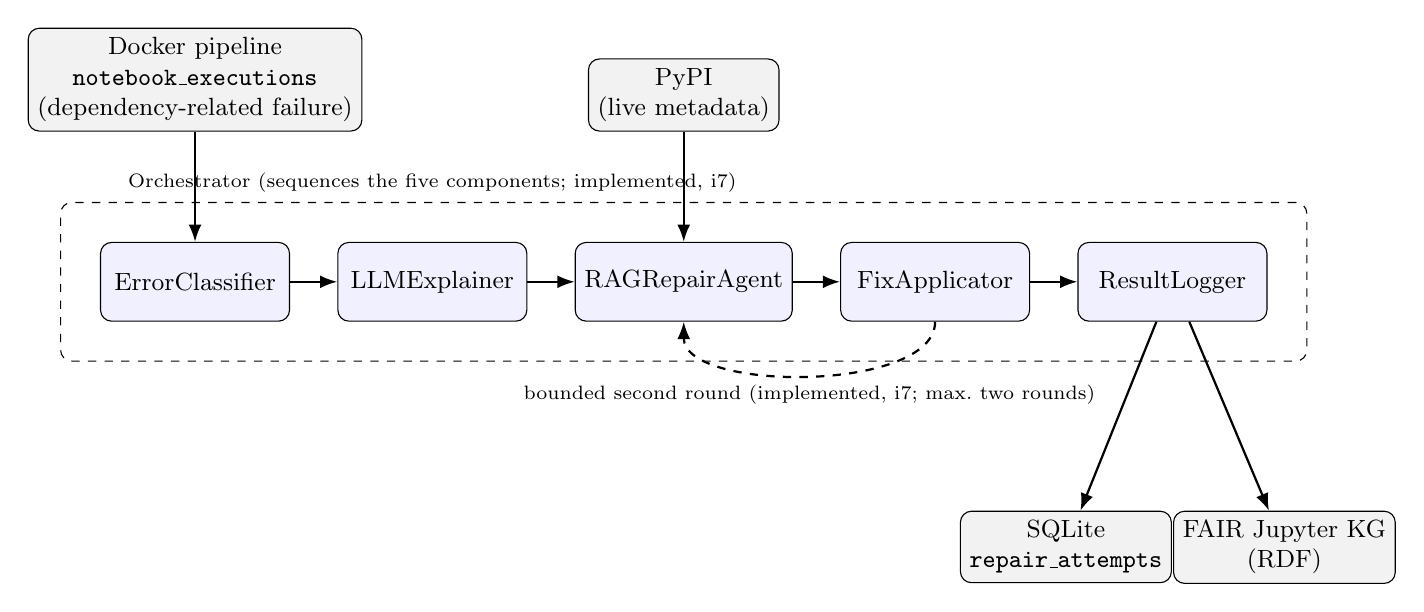
\begin{tikzpicture}[
      font=\small,
      comp/.style={draw, rounded corners, fill=blue!6, minimum width=2.4cm,
                   minimum height=1cm, align=center, node distance=6mm},
      ext/.style={draw, rounded corners, fill=gray!10, minimum width=2.4cm,
                  minimum height=0.9cm, align=center, node distance=6mm},
      arr/.style={-{Latex[length=2.2mm]}, thick},
      darr/.style={-{Latex[length=2.2mm]}, thick, dashed},
    ]
    % five sequenced components
    \node[comp] (ec) {ErrorClassifier};
    \node[comp, right=of ec] (le) {LLMExplainer};
    \node[comp, right=of le] (ra) {RAGRepairAgent};
    \node[comp, right=of ra] (fa) {FixApplicator};
    \node[comp, right=of fa] (rl) {ResultLogger};

    % input above the chain
    \node[ext, above=14mm of ec] (input) {Docker pipeline\\\texttt{notebook\_executions}\\(dependency-related failure)};
    % PyPI above RAGRepairAgent
    \node[ext, above=14mm of ra] (pypi) {PyPI\\(live metadata)};
    % outputs well below ResultLogger, clear of the feedback curve
    \node[ext, below left=24mm and -12mm of rl] (sql) {SQLite\\\texttt{repair\_attempts}};
    \node[ext, below right=24mm and -12mm of rl] (kg) {FAIR Jupyter KG\\(RDF)};

    \draw[arr] (input) -- (ec);
    \draw[arr] (ec) -- (le);
    \draw[arr] (le) -- (ra);
    \draw[arr] (pypi) -- (ra);
    \draw[arr] (ra) -- (fa);
    \draw[arr] (fa) -- (rl);
    \draw[arr] (rl) -- (sql);
    \draw[arr] (rl) -- (kg);

    % bounded second-round feedback path (implemented, i7 - see
    % scripts/run_pipeline.py and sec:orchestrator)
    \draw[darr] (fa.south) .. controls +(0,-9mm) and +(0,-9mm) .. (ra.south)
      node[midway, below, font=\scriptsize] {bounded second round (implemented, i7; max.\ two rounds)};

    % orchestrator: dashed enclosure around the five sequenced components only
    \node[draw, dashed, rounded corners, inner sep=5mm, fit=(ec)(le)(ra)(fa)(rl)] (orch) {};
    % caption placed above LLMExplainer's column, clear of the input and PyPI arrows
    \node[font=\scriptsize, anchor=south] at (le.north |- orch.north)
      {Orchestrator (sequences the five components; implemented, i7)};
  \end{tikzpicture}%
  }
  \caption{Component architecture of the repair layer. The Docker pipeline's
           residual dependency failures enter at the left; the five
           components are sequenced by the orchestrator (dashed enclosure),
           implemented in \texttt{scripts/run\_pipeline.py} and validated by a
           small real pilot (\Cref{sec:orchestrator}); RAGRepairAgent queries
           PyPI for live metadata; ResultLogger writes both the SQLite
           benchmark table and the FAIR Jupyter knowledge graph. The dashed
           feedback arrow is the bounded second round, also implemented and
           capped at two rounds total. The full 187-row evaluation run over
           this pipeline remains future work (\Cref{chap:future-work}).}
  \label{fig:architecture-components}
\end{figure}

Each component is defined below by its responsibility and its input/output
contract. Implementation is deferred to \Cref{chap:methodology}.

\subsection{ErrorClassifier (FR1)}
\label{subsec:errorclassifier}
\textbf{Responsibility.} Decide whether a failure is an in-scope,
pip-fixable dependency error and, if so, extract the failing module and
its sub-type. It reuses the pipeline's existing \texttt{error\_category}
tag as a first filter and refines from \texttt{error\_type} and
\texttt{error\_message}.\\
\textbf{Input.} A \texttt{notebook\_executions} row (the fields listed in
Section~\ref{sec:integration-point}).\\
\textbf{Output.} A classification
$\{\texttt{failing\_module},\ \texttt{subtype},\ \texttt{scope\_status}\}$
where $\texttt{subtype} \in \{\texttt{missing\_package},\
\texttt{wrong\_version},\ \texttt{system\_library},\
\texttt{mapping\_unknown}\}$ and $\texttt{scope\_status} \in
\{\texttt{usable},\ \texttt{excluded}\}$.

\textbf{Explanation is not gated by scope.} \texttt{scope\_status} decides
whether RAGRepairAgent and FixApplicator run on a row, not whether
LLMExplainer does. Every classified row, including an \texttt{excluded} one,
is still passed to LLMExplainer: a researcher whose failure falls outside
the pip-only repair scope still deserves an explanation of what went wrong.
An earlier draft of this chapter placed one shared gate in front of both
LLMExplainer and RAGRepairAgent; \Cref{chap:problem-dataset} and
\Cref{chap:methodology} explain why that was corrected once the repair
component's implementation made the distinction concrete.

\subsection{LLMExplainer (O1)}
\label{subsec:llmexplainer}
\textbf{Responsibility.} Generate a plain-language explanation of the
error for a non-expert reader (NFR2).\\
\textbf{Input.} The error context (error type, message, failing module,
relevant cell).\\
\textbf{Output.} An explanation string and the identifier of the model
that produced it (\texttt{model\_used}), forwarded to the ResultLogger
for logging in \texttt{repair\_attempts.llm\_model}.\\
\emph{The prompt template and model are defined in
\Cref{chap:methodology}; this component's contract is fixed here, its
prompt internals are not.}

\subsection{RAGRepairAgent (O2)}
\label{subsec:repairagent}
\textbf{Responsibility.} Derive a concrete fix for the classified error.
Following PLLM~\cite{bartlett2025pllm},
the suggestion is grounded in live PyPI metadata so that version numbers
are retrieved rather than hallucinated.\\
\textbf{Input.} The classified record (error context, \texttt{failing\_module}),
the repository's requirements and import statements, the injected
model/prompt configuration, and -- in two-round mode -- the prior failed
attempt's new error as optional context.\\
\textbf{Output.} A \emph{fix object} (Section~\ref{subsec:fix-object}).\\
\emph{How PyPI is queried -- endpoints, fields consumed, import-name vs.
install-name resolution, and version selection -- is described in
\Cref{sec:m-repair}. This chapter fixes only the output contract (the fix
object); \Cref{sec:m-repair} also gives the exact field names the
implementation persists, which differ from the illustrative object shown in
Section~\ref{subsec:fix-object} below.}

\subsection{FixApplicator (O3)}
\label{subsec:fixapplicator}
\textbf{Responsibility.} Apply the fix object's command inside an
environment equivalent to the one the repository originally failed in, and
re-execute the notebook to validate it. The notebook is re-run \emph{top to
bottom}, not from the failing cell, because notebook statefulness means a
partial re-run cannot establish that the fix is correct~\cite{grotov2024debug}.\\
\textbf{Input.} A fix object, re-joined against the originating
notebook/repository record, and a rebuilt container equivalent to the one
the failure originally occurred in (\Cref{sec:m-fixapply} explains why this
is a rebuilt environment rather than a reused one, and why the join is
needed).\\
\textbf{Output.} An outcome
$\in \{\texttt{fixed},\ \texttt{still\_failing},\ \texttt{apply\_error}\}$,
together with the new error type/message if the notebook still fails.

\subsection{ResultLogger (O4, O6)}
\label{subsec:resultlogger}
\textbf{Responsibility.} Persist the complete attempt and enrich the
knowledge graph.\\
\textbf{Input.} The classification, explanation, fix object, outcome, and
run metadata.\\
\textbf{Output.} One \texttt{repair\_attempts} row
(Section~\ref{subsec:repair-table}) and, via the RML mapping, the
corresponding RDF triples (Section~\ref{subsec:kg}). The benchmark
dataset (O4) and the KG enrichment (O6) are both produced from this
single component.\\
\emph{This contract was built and validated by the result-logging and
knowledge-graph implementation (\Cref{sec:m-resultlogger}), including how
the four upstream JSONL outputs are actually joined -- a detail this
chapter leaves unspecified, since a join strategy is an implementation
concern, not a contract one -- and checked against real pilot data
(\Cref{sec:v-i6}).}

% ---------------------------------------------------------------------
\section{Orchestration and Control Flow}
\label{sec:orchestrator}

The orchestrator iterates over the target rows and runs the components in
order: classify, explain, repair, apply, log. Three properties are fixed
at this level.

% TODO-FULL-RUN: update after full orchestrated dataset execution
\fullrunupdate{The orchestrator described below is now implemented
(\texttt{scripts/run\_pipeline.py}) and validated by a small real pilot run
against real Ollama, PyPI, and Docker, recorded in the accompanying
implementation documentation (\texttt{docs/pipeline-orchestrator.md}) --
not the full 200-row usable set. Each of ErrorClassifier through ResultLogger exists,
is independently tested, and is called by the orchestrator exactly as
described below, including the bounded two-round feedback mode described
later in this section. What remains is the full 200-row usable-set
run itself, the resulting one-round-vs-two-round comparison, and full
benchmark/knowledge-graph population from it -- \Cref{chap:future-work}.
Result logging and knowledge-graph enrichment were already implemented
before the orchestrator (\Cref{sec:m-resultlogger}) and are unchanged by
it; the orchestrator only calls them.}

\paragraph{Round switch.}
The default is a single repair round. In two-round mode, if the outcome is
\texttt{still\_failing}, the new error is fed back to the RAGRepairAgent
once more and the resulting fix is re-applied before the attempt is
logged. This feedback structure follows the re-execution-driven repair of
ChatRepair~\cite{xia2024chatrepair};
the one- versus two-round comparison is the subject of the ablation study.

\paragraph{Failure isolation (NFR4).}
Every attempt is logged, even when a component itself errors -- malformed
LLM output, an unreachable PyPI, or a re-execution timeout. Such cases are
caught and recorded with the appropriate \texttt{outcome}; a single
problematic notebook never aborts the batch.

\paragraph{Configuration surface (NFR5).}
The model, the prompt strategy, and the round count are injected per run
rather than hard-coded, so they can be swapped without changing component
code. The same injection points drive the model and prompt comparisons in
the evaluation.

\begin{verbatim}
for row in notebook_executions where error_category = 'DEPENDENCY_ERROR':
    cls = ErrorClassifier(row)
    if not cls.is_dependency_error:
        continue
    explanation = LLMExplainer(row, cls)            # O1
    fix         = RAGRepairAgent(row, cls)          # O2  (PyPI-grounded)
    outcome     = FixApplicator(fix, container)     # O3  (re-run top-to-bottom)
    log(row, cls, explanation, fix, outcome, round=1)

    if two_round and outcome == 'still_failing':    # second round
        fix2     = RAGRepairAgent(row, cls, prev_error=outcome.new_error)
        outcome2 = FixApplicator(fix2, container)
        log(row, cls, explanation, fix2, outcome2, round=2)
\end{verbatim}
% LISTING: switch the block above to lstlisting/algorithm if available.

% ---------------------------------------------------------------------
\section{Data Contracts}
\label{sec:data-contracts}

\subsection{Fix Object}
\label{subsec:fix-object}

The RAGRepairAgent emits the \emph{proposed} fix as structured JSON,
before application. Version~1 is pip-only: \texttt{action} is one of
\texttt{install}, \texttt{pin\_version}, or \texttt{none}; \texttt{version}
is \texttt{null} for a plain install; and \texttt{command} is exactly what
the FixApplicator runs inside the container. Notebook-code edits
(\texttt{replace\_import}) are deferred to future work -- in practice many
renamed-import cases are still resolved by pinning an older version where
the import was valid, which remains a pip fix.

\emph{This is the object's conceptual shape, fixed at design time.} The
implemented object (\Cref{sec:m-repair}) keeps the same four meaningful
values -- action, resolved install name, version, and the evidence behind
them -- but names and nests the fields differently
(\texttt{final\_action}, \texttt{final\_install\_name}, and so on, with
retrieval evidence in a separate \texttt{retrieval\_result} block) once the
validation logic in \Cref{sec:m-repair} was actually built. The example
below should be read as the contract's intent, not as the literal persisted
record.

\begin{verbatim}
{
  "action": "pin_version",
  "import_name": "scanpy",
  "install_name": "scanpy",
  "version": "1.9.3",
  "command": "pip install scanpy==1.9.3",
  "rationale": "Notebook needs an API present only up to 1.9.x; pinning the
                last compatible release.",
  "pypi_evidence": {
    "latest_version": "1.10.1",
    "chosen_version": "1.9.3",
    "requires_python": ">=3.9"
  }
}
\end{verbatim}
% LISTING: JSON

\subsection{The \texttt{repair\_attempts} Table}
\label{subsec:repair-table}

The repair layer writes to a single new SQLite table,
\texttt{repair\_attempts}, which serves a dual purpose: it is the live
validation log (O3) and the reusable benchmark dataset (O4). It records
\emph{one row per attempt}: a two-round repair produces two rows, and
re-running the same targets under a different model or prompt produces
further rows. The error data is never copied -- each row joins back to the
originating failure via \texttt{notebook\_execution\_id}. Filtering on
\texttt{round}, \texttt{llm\_model}, \texttt{prompt\_strategy}, and
\texttt{run\_id} is what powers the ablation and the model/prompt
comparisons.

\begin{verbatim}
CREATE TABLE repair_attempts (
  id                      INTEGER PRIMARY KEY,
  notebook_execution_id   INTEGER NOT NULL,   -- FK -> notebook_executions.id

  -- from ErrorClassifier
  failing_module          TEXT,               -- e.g. "scanpy"
  subtype                 TEXT,               -- missing_package | wrong_version

  -- from LLMExplainer (O1)
  explanation             TEXT,

  -- from RAGRepairAgent -- the proposed fix (O2)
  action                  TEXT,               -- install | pin_version | none
  install_name            TEXT,               -- resolved PyPI name
  version                 TEXT,               -- version to pin, or NULL
  command                 TEXT,               -- exact command run
  rationale               TEXT,
  pypi_evidence           TEXT,               -- JSON: versions seen, requires_python

  -- from FixApplicator -- the outcome (O3)
  outcome                 TEXT,               -- fixed | still_failing | apply_error
  new_error_type          TEXT,
  new_error_message       TEXT,

  -- run metadata (for experiments)
  llm_model               TEXT,
  prompt_strategy         TEXT,               -- for the prompt-strategy comparison
  round                   INTEGER,            -- 1 or 2 (the ablation)
  run_id                  TEXT,               -- groups one run / config
  created_at              TEXT,

  FOREIGN KEY (notebook_execution_id) REFERENCES notebook_executions(id)
);
\end{verbatim}
% LISTING: SQL

The result-logging implementation built this table exactly as specified here:
\texttt{scripts/result\_logger.py}'s own \texttt{CREATE TABLE} statement
reproduces this nineteen-column schema unchanged, the one data contract in
this chapter that implementation did not have to revise once it was actually
built. \Cref{sec:m-resultlogger} describes how each of the eighteen
non-\texttt{id} columns is populated from the four upstream JSONL files,
including how a \texttt{notebook\_execution\_id} that legitimately repeats
across separate attempts is kept as separate rows rather than collapsed.

\subsection{Knowledge-Graph Enrichment}
\label{subsec:kg}

The FAIR Jupyter knowledge graph~\cite{samuel2024fairkg}
is not written by hand; it is generated from per-table RML mappings
(\texttt{*.rml.ttl}) run by the existing build script
(\texttt{run\_fairjupyter\_kg.sh}), using Morph-KGC as the mapping engine.
Objective~O6 adds a single mapping, \texttt{repair\_attempts.rml.ttl},
modelled on the existing \texttt{mapping/rml\_mapping/executions.rml.ttl}. It
re-expresses each \texttt{repair\_attempts} row as triples and attaches them
to the notebook node already present in the graph, so that repair history
becomes queryable alongside the existing reproducibility data. This mapping
follows the existing FAIR Jupyter knowledge-graph architecture -- CSV-based
RML mappings run through Morph-KGC -- rather than introducing a separate
RDF-generation pipeline of its own.

The vocabulary strategy follows the earlier design notes: \emph{reuse} existing
\texttt{repr:} terms where they already fit (e.g.\ \texttt{repr:exception}),
\emph{add} new \texttt{repr:} terms for repair-specific facts, and use
PROV-O~\cite{provenance2013}
for the activity/agent/time layer, representing each repair as a
\texttt{prov:Activity}. This serialisation of repair provenance directly
serves the Reusable principle of FAIR~\cite{wilkinson2016fair} and the
execution-environment provenance emphasised by
FAIR4RS~\cite{barker2022fair4rs}.
The base IRI is \texttt{repr:}~$=$~\url{https://w3id.org/reproduceme/} and
the serialisation is Turtle (\texttt{.ttl}).

\begin{verbatim}
repr:notebook_512  repr:hadRepairAttempt  repr:repairattempt_001 .

repr:repairattempt_001
    a                       prov:Activity, repr:RepairAttempt ;
    repr:exception          "ModuleNotFoundError" ;   # reuse existing term
    repr:failingModule      "scanpy" ;                # new term
    repr:appliedFix         "pip install scanpy==1.9.3" ;
    repr:fixOutcome         "fixed" ;
    prov:wasAssociatedWith  repr:codellama_13b ;       # which model did it
    prov:endedAtTime        "2026-07-15T14:22:00Z"^^xsd:dateTime .
\end{verbatim}
% LISTING: Turtle. NOTE: this is the mapping's design-time intent, not its
% literal implemented shape. The implemented mapping (\Cref{sec:m-resultlogger})
% keeps the same reuse-vs-add vocabulary strategy and the same
% prov:endedAtTime typing, but does not use repr:appliedFix or
% prov:wasAssociatedWith, and reuses repr:exception/repr:msg for the
% post-repair error rather than the original one, which the existing
% executions mapping already records; the exact predicate names actually
% generated are listed there.

% ---------------------------------------------------------------------
\section{Scope and Forward References}
\label{sec:arch-scope}

This chapter fixes the component contracts, the orchestration logic, and
the three data contracts (fix object, \texttt{repair\_attempts} table, KG
mapping). The following are covered elsewhere in this thesis, or remain
future work:

\begin{itemize}
  \item Prompt templates and open-model selection -- \Cref{sec:m-explanation,sec:m-repair}.
  \item PyPI retrieval internals: endpoints, consumed fields, import-name
        vs.\ install-name resolution, and version selection --
        \Cref{sec:m-repair}.
  \item Component implementation, the real data shapes produced, and the
        design deviations discovered while building them, including how
        ResultLogger joins the four upstream outputs and how the
        knowledge-graph mapping was implemented -- \Cref{chap:methodology};
        their validation against real pilot data -- \Cref{chap:validation}.
  \item Full end-to-end orchestration and the bounded two-round feedback
        mode -- \textbf{implemented} (\texttt{scripts/run\_pipeline.py});
        the full 200-row usable-set run and the resulting
        one-round-vs-two-round comparison remain future work -- see
        \Cref{chap:future-work}.
\end{itemize}


%---------------------------------------------------------
% Chapter 5: Methodology and Implementation
%---------------------------------------------------------
\chapter{Methodology and Implementation}
\label{chap:methodology}

\Cref{chap:architecture} fixed what each component is responsible for and
what data it exchanges with its neighbours. This chapter explains how each
component was built: the concrete rules and libraries used, and the reasons
behind the decisions that shaped them.

The chapter follows the order data actually moves through the system. The
working dataset is prepared first. Then come classification and context
extraction, the explanation component, the PyPI-grounded repair component,
and fix application. The orchestrator that drives these components in a
single unattended pass, and that carries a newly exposed error into the
bounded second round, is described next, because its behaviour is what
the evaluation measures. Result logging and knowledge-graph enrichment
come last, because they join the outputs of every earlier component into
one persistent record.

\section{Implementation Overview}
\label{sec:m-overview}

This section gives one condensed view of how the stages connect, so that
the detail in the rest of the chapter does not obscure how the pieces form
a single system.

\begin{verbatim}
Docker-pipeline dependency-error dataset (214 rows)
  -> dataset preparation      scripts/prepare_dependency_dataset.py
  -> context extraction /
     classification           scripts/extract_error_contexts.py
  -> LLMExplainer             scripts/run_llm_explainer.py
  -> RAGRepairAgent           scripts/rag_repair_agent.py
  -> FixApplicator            scripts/fix_applicator.py
  -> new error: reclassify, explain,
     repair if eligible (round 2)  scripts/run_pipeline.py
  -> ResultLogger (SQLite)    scripts/result_logger.py
  -> CSV export               scripts/export_repair_attempts_csv.py
  -> RML mapping (Morph-KGC)  repair_attempts.rml.ttl
  -> repair RDF linked to FAIR Jupyter KG notebook IRIs
\end{verbatim}

Each arrow is a data hand-off: a plain file, a database, or a call between
the components' own functions. Every stage can be invoked as its own script
against the previous stage's output, which is how each was developed and
tested. The same stages are also driven in sequence by a single
orchestrating process (\texttt{scripts/run\_pipeline.py}) within one pass,
which is how the evaluation in \Cref{chap:validation} was run.

The sections below follow this order, one component at a time.
\Cref{sec:m-worked-example} then traces one concrete record through every
stage.

\section{Dataset Preparation}
\label{sec:m-dataset}

\Cref{chap:problem-dataset} already gave the resulting numbers for this
stage: 214 dependency-error rows, 200 usable and 14 excluded, split 13/187
between development and evaluation. This section explains how
\texttt{scripts/prepare\_dependency\_dataset.py} produces those numbers, and
why the rules behind them were chosen.

The script reads the Docker pipeline's own \texttt{notebook\_executions}
table, and keeps every row where \texttt{error\_category =
'DEPENDENCY\_ERROR'}. For each kept row, it applies two independent
decisions, deterministically and without any LLM involvement. The
first is a \emph{subtype}: is the module missing entirely, present but
incompatible, a missing system library, or an ambiguous local name? The
second is a \emph{scope status}: is this row inside the pip-only v1
repair scope at all? Both decisions rely only on simple, inspectable
rules over the \texttt{error\_type} and \texttt{error\_message} fields
the Docker pipeline already recorded. For example, a message containing
\texttt{".so"} or "shared object file" is classified as
\texttt{system\_library}. A failing module name drawn from a short list
of known-ambiguous names (\texttt{utils}, \texttt{statistics},
\texttt{config}, \texttt{helpers}, \texttt{src}) is classified as
\texttt{mapping\_unknown}.

Doing this filtering with plain rules, before any language model is
involved, was a deliberate choice. A decision that determines whether a
row is even eligible for automated repair should be explainable and
reproducible on its own terms. An LLM's judgement about scope
eligibility would be harder to audit, and could silently change between
runs of the same model. Keeping this gate deterministic also means
every later component can trust \texttt{scope\_status} directly,
instead of re-deriving eligibility itself.

The dataset is also split into three disjoint groups: 13 rows set aside
for manually designing and sanity-checking the explanation and repair
prompts (\Cref{sec:m-explanation,sec:m-repair}), 187 usable rows
reserved for a later, controlled evaluation run, and the 14 excluded
rows. Separating a small development sample from the evaluation set
matters for the same reason it matters in any machine-learning
setting. A prompt tuned by looking at a specific row, and then tested
again on that same row, would give an optimistic and misleading
impression of how well the prompt generalises.

The script writes four output files: a CSV of the classified rows, a schema
document describing every column, a statistics file with the counts used
throughout this thesis, and a split-manifest file recording exactly which
notebook execution IDs fall into which split, so the same split can be
reproduced later rather than re-randomised.

\section{Context Extraction and Error Classification}
\label{sec:m-classification}

\texttt{scripts/extract\_error\_contexts.py} takes each dataset row
prepared above and adds two things: a more detailed root-cause hint
with a confidence level, and, where possible, the actual source code
around the failure. Every field the dataset-preparation stage already
computed (\texttt{scope\_status}, \texttt{exclusion\_reason},
\texttt{split}) is carried through unchanged. This stage enriches
every row regardless of scope, so an excluded row still receives full
context for its explanation.

\subsection{Root-Cause Hints}

The subtype produced by dataset preparation is refined into one of seven
root-cause hints:

\begin{itemize}
  \item \texttt{direct\_missing\_package} -- the module is genuinely absent;
  \item \texttt{import\_distribution\_name\_mismatch} -- the import name
        differs from its PyPI distribution name, for example
        \texttt{sklearn} versus \texttt{scikit-learn};
  \item \texttt{version\_or\_api\_incompatibility} -- a "cannot import name"
        style failure;
  \item \texttt{transitive\_dependency} -- a generic \texttt{ImportError}
        not matching a more specific pattern;
  \item \texttt{system\_level\_dependency} -- a missing shared library;
  \item \texttt{local\_import\_or\_path\_issue} -- an ambiguous local module
        name; and
  \item \texttt{insufficient\_context} -- not enough information to decide.
\end{itemize}

Each hint also carries a confidence level. A direct pattern match gives
high confidence: a missing-module message, a "cannot import name" message,
or a \texttt{.so} failure. Softer phrasing, such as an "install" or
"required" hint, gives medium. An ambiguous local module, or a message
carrying too little information to decide, gives low.

\subsection{Recovering Source Context}

Three sources of context are used, ordered by reliability. The first is a
legacy execution table from an earlier pipeline run. Because this table
was not produced by the same execution as the current dataset and has no
timestamp, it is treated only as supporting evidence.

A legacy row is accepted only when its final reported error matches the
current failure. Matching only the notebook or the failing module name is
not enough. For example, a cell may import both \texttt{pandas} and
\texttt{sklearn}, but fail on \texttt{pandas} in one execution and on
\texttt{sklearn} in another. Treating those as the same failure would
attach the wrong source context.

In practice, 162 of the 214 dataset rows (76\%) have a matching notebook
ID in the legacy table, but only about 40\% of those records contain the
correct failing module in the stored traceback. For this reason, legacy
context is used only as a low-confidence hint and is never trusted on its
own.

The second tier, used only when explicitly requested, fetches the
notebook and its dependency files directly from GitHub. It uses the
repository's recorded commit where available, and falls back to the
\texttt{main} or \texttt{master} branch otherwise. The third tier
falls back to the metadata already present from dataset preparation
(error type, message, cell index, failing module), when no source can
be recovered at all. This is unavoidable here: the repositories cloned
during the original Docker pipeline run were never kept on this
machine, so no local copy of any notebook's source exists unless it is
fetched again.

\subsection{Limitations}

A few limitations follow directly from the above, and are worth stating
plainly, because they affect how confidently later components can rely
on this context. Remote fetching is not pinned to the exact commit that
originally failed, unless that commit happens to still be resolvable.
So a freshly fetched notebook can, in rare cases, differ slightly from
the one that actually produced the recorded error.
\texttt{error\_cell\_index} indexes into the notebook's full cell list,
so a notebook edited since the original run can shift cell positions
and misalign the index. Any unexpected per-row failure (a malformed
row, a database error) falls back to a bare metadata-only record,
rather than aborting the whole batch -- this keeps one bad row from
blocking the other 213.

\section{LLM Explanation Component}
\label{sec:m-explanation}

LLMExplainer (\Cref{subsec:llmexplainer}) turns a classified failure into a
plain-language account of what went wrong. It is the component most
directly tied to the thesis title, and its role is deliberately narrow: it
explains a failure, it never proposes how to fix one.

\subsection{Role and Separation from Repair}
\label{sec:m-explanation-role}

The prompt sent to the model instructs it to describe the failure in plain,
non-technical language, using only the information supplied, and explicitly
forbids it from suggesting a fix -- deriving a repair is RAGRepairAgent's
job, kept structurally separate (\Cref{sec:m-repair}). This separation
serves two purposes. First, it keeps each component's failure mode
contained: an explanation that misjudges a detail is a readability problem,
while a repair suggestion that misjudges a package name or version is
executed inside a container, so the two carry very different risk and
deserve very different validation. Second, it lets LLMExplainer's scope be
wider than RAGRepairAgent's: the pip-only repair scope defined in
\Cref{sec:pd-scope} restricts which rows may be \emph{repaired}, not which
rows may be \emph{explained} (\Cref{sec:pd-explanation-scope}). A researcher
whose notebook fails because of a missing system library still receives a
plain-language explanation of the failure, even though the current repair
layer cannot act on that particular case.

The same two principles carry over to the second repair round. When a
repaired notebook fails again on a new error, that error is reclassified
and explained as a record of its own before its repair eligibility is
evaluated, so the reader receives an account of every error the pipeline
encountered, not only the first (\Cref{sec:m-orchestrator-round2}). The
explainer is called with the same prompt, schema, and retry rule in both
rounds; the round only changes which record it is given.

\subsection{Model and Runtime Selection}

The explanation and repair components share one open, locally-run
model, rather than each using a different one. \textbf{Gemma-2 9B} was
selected as the primary model because PLLM~\cite{bartlett2025pllm}, the
closest prior system, reports Gemma-2 9B with RAG as its own
best-performing configuration for exactly this kind of dependency task.
Using the same model for both explanation and repair keeps a later
comparison between configurations clean: any difference in outcome can
be attributed to the prompt or the retrieval design, not to a hidden
difference in which model produced which part of the result.
CodeLlama-13B and DeepSeek-Coder (7B and 13B) were kept as fallback
candidates, motivated by Szalontai et al.~\cite{szalontai2024codellama}
and a broader empirical comparison of code-specialised
models~\cite{empiricalapr2025}. Both report that smaller,
code-specialised models can match or beat larger general-purpose ones on
repair tasks. Neither fallback was needed: Gemma-2 9B performed adequately
in the sanity checks run on the development split. A separate experiment
later replaced Gemma with a much larger open model to test how much the
choice mattered (\Cref{sec:v-model-sensitivity}).

Ollama was chosen as the serving runtime because it gives simple local
access to a quantised model without setting up a GPU-serving stack, which
is appropriate for a component running one notebook at a time rather than
serving high-throughput traffic. A hardware check confirmed \texttt{gemma2:9b}
runs on the available machine using 6.3~GB of memory, entirely on CPU, with
a 4096-token context window -- workable, though slow, which later became
relevant to a timeout decision described in \Cref{sec:m-repair}.

\subsection{Structured Explanation Output}
\label{sec:m-explanation-deviation}

An explanation is read by a person, but it also has to be logged,
validated, and processed by later stages. Free prose cannot be checked
automatically for the fields those stages need. The explainer therefore
returns a single JSON object, validated against a fixed schema
(\texttt{schemas/}\allowbreak\texttt{explanation.schema.json}) with exactly
six fields:

\begin{itemize}
  \item \texttt{summary} -- a short, plain-language statement of what failed;
  \item \texttt{root\_cause} -- why it failed, in the same plain language;
  \item \texttt{evidence} -- a list of the concrete signals the explanation
        is grounded in (the error type, the error message, the root-cause
        hint);
  \item \texttt{failing\_module} -- the module named in the explanation;
  \item \texttt{explanation\_confidence} -- \texttt{high}, \texttt{medium},
        or \texttt{low}; and
  \item \texttt{limitations} -- what the explanation could not determine,
        for example because only metadata, not source code, was available.
\end{itemize}

The plain-language requirement is enforced inside the fields rather than
abandoned: \texttt{summary} and \texttt{root\_cause} are what a reader
sees, and the prompt still constrains them to short, non-technical
sentences. The surrounding structure exists for the pipeline, not for the
reader. This follows the same pattern used for the repair prompt
(\Cref{sec:m-repair}).

The schema's \texttt{explanation\_confidence} field is named differently
from the classifier's own \texttt{confidence} field
(\Cref{sec:m-classification}) because the two measure different things and
can legitimately disagree. A classifier can be highly confident it matched
a known pattern while the model is only moderately confident it has
explained the underlying cause correctly.

\subsection{Prompt, Validation, and Retry}

The prompt instructs the model to write in plain, non-technical language,
to use only the information supplied, and never to suggest a fix. Using
only supplied information means never inventing a version number, a file
name, or a cause not visible in the error. The runner sends
this prompt to \texttt{gemma2:9b} through Ollama (or, in the
model-sensitivity run of \Cref{sec:v-model-sensitivity}, to Qwen through
the same provider interface with the same prompt), parses the response as
JSON, and validates it against the schema. Each request has a 120-second
timeout. On invalid JSON, a schema violation, a timeout, or an unavailable
model, the runner retries once with a corrective prompt. If the second
attempt also fails, the failure itself is logged, with its category
(\texttt{timeout}, \texttt{model\_unavailable}, or a validation failure),
rather than discarded, so no row silently disappears from the results
file. The evaluation in \Cref{chap:validation} keeps these categories
apart: a request that timed out is a runtime failure of the model service,
not a malformed model output, and the two are reported separately.

Each logged result keeps three things apart: the input metadata from the
classification stage, the model and prompt configuration used, and the
generated explanation with its validation status, latency, and retry count.
Separating them means a later reader cannot confuse the original error text
with text the model wrote about it. It also lets the result-logging stage
(\Cref{sec:m-resultlogger}) join an explanation back to its originating
notebook by \texttt{notebook\_execution\_id} alone.

\subsection{A Real Explanation Record}
\label{sec:m-explanation-example}

The following committed record illustrates the schema above on a real,
already-classified failure: \texttt{notebook\_execution\_id}~8, a
\texttt{ModuleNotFoundError} for \texttt{sklearn}.

\begin{quote}
\small
\begin{sloppypar}
\textbf{summary:} "The notebook execution failed because Python could not
find the module 'sklearn'."\\[2pt]
\textbf{root\_cause:} "The notebook imports 'sklearn', which is not
available in the execution environment. The classifier also marks this as
an import/distribution-name mismatch, meaning the import name may not
directly match the package distribution name."\\[2pt]
\textbf{evidence:} ["The error type is ModuleNotFoundError.", "The error
message says: No module named 'sklearn'.", "The root\_cause\_hint is
import\_\allowbreak distribution\_\allowbreak name\_\allowbreak mismatch."]\\[2pt]
\textbf{failing\_module:} "sklearn"\\[2pt]
\textbf{explanation\_confidence:} "high"\\[2pt]
\textbf{limitations:} "Only metadata is available, so the exact failing
cell and dependency files cannot be inspected."
\end{sloppypar}
\end{quote}

This record was generated with the \texttt{few\_shot} prompt strategy. It
succeeded on the first attempt and required 98{,}029~ms on the CPU-only
hardware described above. The example is included only to illustrate the
structure of a real explanation record; it should not be interpreted as
evidence of explanation quality across the full dataset.
The few-shot prompt contains two fixed examples in\\
\texttt{prompts/dependency\_explanation\_v1.txt}:
this \texttt{sklearn}/\texttt{ModuleNotFoundError} case and the
\texttt{scipy}/\texttt{cumtrapz} case discussed in
\Cref{sec:m-worked-example}. Both examples come from the 13-row development
split and remain unchanged for every LLM call. No example from the reserved
evaluation split is included in the prompt.


\section{PyPI-Grounded Repair Generation}
\label{sec:m-repair}

RAGRepairAgent (\Cref{subsec:repairagent}) does not install anything. Its
only job is to answer one question -- \emph{what repair should be
attempted?} -- and to answer it safely: never inventing a package name,
never inventing a version number, and never handing a later component a raw
string to execute in a shell. This section explains how that is achieved.

\subsection{Overall Flow}

\begin{verbatim}
classified dependency failure (usable)
    -> identify the failing import
    -> resolve the import name to a PyPI distribution name
    -> query the PyPI registry for that distribution
    -> filter the returned versions to a small, safe candidate set
    -> for a version-incompatibility failure, intersect with
       curated compatibility evidence
    -> give the LLM only this grounded candidate set
    -> validate the LLM's proposal against the same evidence
    -> if valid, deterministically build the exact install command
\end{verbatim}

The design principle behind this flow is that the language model is never
the only thing standing between an error message and a command that will
later run inside a container. Four separate layers each have exactly one
job, and each layer only trusts what the previous layer has already
verified.

\subsection{Layer 1: Deterministic Retrieval}
\label{sec:m-repair-retrieval}

Before any network request, the failing Python import name must be
resolved to an installable PyPI distribution name. The two are
frequently different: \texttt{sklearn} installs as
\texttt{scikit-learn}, \texttt{cv2} as \texttt{opencv-python},
\texttt{skimage} as \texttt{scikit-image}, \texttt{umap} as
\texttt{umap-learn}, \texttt{pkg\_resources} as \texttt{setuptools}, and
\texttt{Bio} as \texttt{biopython}. A small, explicit, hand-curated
mapping table (\texttt{config/package\_mapping.yaml}) holds every case
the retriever is allowed to resolve. An import name absent from this
table is never assumed to also be its own package name. Instead, the
retriever reports a \texttt{mapping\_unknown} status, without making
any PyPI request at all. This rule matters concretely for this
thesis's own dataset: \texttt{sklearn} and \texttt{pkg\_resources} are,
respectively, the second and first most common failing modules
(\Cref{tab:pd-top-modules}). Getting this mapping right or wrong
affects a large share of the dataset, not an edge case.

Once resolved, the distribution's release metadata is retrieved from the
official PyPI JSON Simple API
(\texttt{GET /simple/\{distribution\}/}), normalising the name first
according to PEP 503. This endpoint was chosen deliberately over the older
project JSON endpoint's \texttt{releases} field, which PyPI's own
documentation marks as deprecated for new integrations; the newer endpoint
is the one PyPI recommends going forward. The returned files are grouped by
release version, and a safe candidate set is computed by dropping
unparseable files, pre-releases, and releases where every file is yanked,
and by checking each release's declared \texttt{requires-python} against
the runtime the notebook actually executed under.

That runtime version is a fixed constant, \texttt{"3.10"}
(\texttt{config/rag\_repair.yaml}), not looked up per notebook. This is not
an approximation of convenience: the Docker pipeline builds every
repository's container from the same template, with the base image
hardcoded to \texttt{python:3.10-slim}, so every notebook this component
processes genuinely ran under the same interpreter version. The
notebook's own recorded kernel metadata is deliberately not used as a
substitute, because it reflects what the notebook's original author had
installed, which is frequently stale or missing, not what the Docker
container the notebook actually failed in provides.

The final candidate list is capped to five versions, newest first, to keep
the amount of version metadata placed in the prompt bounded and readable.

\subsection{Why PyPI Metadata Is Not Enough}
\label{sec:m-repair-compat}

For a \texttt{wrong\_version} failure -- a "cannot import name" error --
knowing that a release exists and supports the right Python version is
not enough. PyPI's own Simple API specification (PEP 691) only
exposes, per file, its filename, URL, hashes, required Python version,
size, upload time, and yanked status. It says nothing about which
functions or classes a given release actually provides. Proving that,
for example, \texttt{scipy.integrate.cumtrapz} still exists in a
specific SciPy release requires consulting that project's own
documentation, not PyPI.

This gap is closed with a small, hand-curated compatibility registry. Each
entry records one import symbol, the version range in which an official
source confirms that symbol still exists, and a link to that source. \Cref{tab:m-compat}
lists the three patterns curated for this dataset, all covering symbols
that were removed in a major SciPy or NumPy release.

\begin{table}[htbp]
  \centering
  \begin{tabular}{|p{3.8cm}|p{2.5cm}|p{5.7cm}|}
    \hline
    \textbf{Symbol} & \textbf{Compatible with} & \textbf{Official source} \\
    \hline
    \texttt{scipy.\allowbreak integrate.\allowbreak cumtrapz} & \texttt{<1.14.0} & SciPy 1.14.0 release notes, "Expired deprecations" \\
    \hline
    \texttt{scipy.sparse.\allowbreak sputils.\allowbreak isshape} & \texttt{<1.14.0} & SciPy 1.14.0 release notes, cross-checked against SciPy's source repository \\
    \hline
    \texttt{numpy.\allowbreak Visible\allowbreak Deprecation\allowbreak Warning} & \texttt{<2.0.0} & NumPy 2.0.0 release notes, "NumPy 2.0 Python API removals" \\
    \hline
  \end{tabular}
  \caption{Curated API-compatibility evidence used for \texttt{wrong\_version} repairs.}
  \label{tab:m-compat}
\end{table}

The registry is intentionally small and manually curated. It contains verified
compatibility rules only for the specific wrong-version API failures observed
in this thesis dataset. Each rule was checked against an official source. If a
wrong-version failure is not covered by the registry, the system does not guess
a compatibility rule and therefore abstains from proposing a version-based
repair.
The registry is therefore dataset-specific rather than a general-purpose
compatibility database. Its purpose is to provide reliable evidence for the
wrong-version patterns present in the evaluated corpus.

\subsubsection{Layer 2: What the Model Decides}

After Layer~1 has resolved the package and retrieved the available PyPI
evidence, the repair model chooses a repair from that grounded information.
It receives the classified failure, including the error type and message,
failing module, subtype, and root-cause hint. Where available, the failing
cell source is also included. Layer~1 additionally provides the resolved
distribution name, the Python target, the compatible candidate releases,
and, for wrong-version failures, the applicable compatibility constraint.

The model does not receive the raw PyPI response. Instead, it sees only the
candidate set already filtered by the deterministic retrieval layer. It also
does not receive the LLMExplainer output or repository dependency files such
as \texttt{requirements.txt}; the latter are used later when FixApplicator
reconstructs the execution environment.

The model returns a structured repair proposal with three possible actions:
\texttt{install}, \texttt{pin\_version}, or \texttt{none}. For
\texttt{install}, it identifies the distribution to install. For
\texttt{pin\_version}, it additionally selects a version from the supplied
candidate set. The \texttt{none} action represents abstention when the
available evidence does not support a repair.


\subsection{Layers 3 and 4: Validation and Command Construction}

Before a repair proposal is used, it first passes schema validation and is then 
checked against the evidence retrieved in Layer 1. 
Five deterministic grounding checks are applied:

\begin{sloppypar}
\begin{itemize}

  \item \texttt{action} must be one of the three allowed values:
        \texttt{install}, \texttt{pin\_version}, or \texttt{none}.

  \item A proposed \texttt{install\_name} must exactly match the
        distribution resolved by the retriever.

  \item A proposed \texttt{version} must appear in the supplied
        candidate list.

  \item An \texttt{install} action for a \texttt{missing\_package}
        additionally requires at least one Python-compatible candidate.

  \item A \texttt{pin\_version} action for a \texttt{wrong\_version}
        additionally requires verified compatibility evidence.

\end{itemize}
\end{sloppypar}

The proposal is also checked for unsafe string values, such as whitespace,
leading dashes, or shell metacharacters. If any validation check fails, the
proposal is rejected and the action is set to \texttt{none}. The system does
not replace an invalid package or version with a guessed alternative.

Only validated proposals are converted into executable commands. The command
is constructed deterministically by the pipeline rather than generated by the
LLM. For example, an installation produces
\texttt{python -m pip install <package>}, while a version pin uses
\texttt{<package>==<version>}. This ensures that unrestricted model-generated
text is never executed directly.

If the model response cannot be parsed, fails schema or grounding validation,
times out, or the model is unavailable, the component retries once. The reason
for the failure is included in the retry prompt. If the second attempt also
fails, the component returns \texttt{action: none}, and no repair is applied.

\subsection{Why Repository Dependency Files Are Not Used as Repair Evidence}
\label{sec:m-repair-nodeps}

Repository dependency files such as \texttt{requirements.txt} are useful for
reconstructing an environment, but they are not reliable enough to serve as
direct repair evidence. A declared dependency file does not necessarily
describe the exact package state in which the recorded failure occurred. It
may be incomplete, outdated, unpinned, or may itself contain the version that
caused the incompatibility.

The files are also inconsistent across repositories. Some projects use\\
\texttt{requirements.txt}, while others use \texttt{setup.py},
\texttt{pyproject.toml}, multiple requirement files, or no explicit dependency
file at all. Making repair generation depend on one of these files would
therefore provide different amounts and qualities of evidence for different
notebooks.

For these reasons, the repair decision is based on evidence that can be checked
independently of the repository's declared environment: the observed failure,
the resolved PyPI distribution, available releases, and compatibility evidence
where applicable. Repository dependency files are used later by FixApplicator
when rebuilding the baseline environment in which the proposed repair is
tested.

This separation gives the two kinds of information different roles. Dependency
files describe how the repository expects its environment to be constructed,
whereas the repair evidence is used to determine how the observed dependency
failure should be addressed.

\subsection{Runtime Configuration}

RAGRepairAgent shares its model with the explanation component:
\texttt{gemma2:9b} through Ollama, temperature 0.1, top-p 0.9, and at most
700 generated tokens. The request timeout is 300 seconds. This value was
set from measurement. In a pilot run on the CPU-only hardware described
above, the same repair request timed out twice under an initial 120-second
limit and then succeeded at the first attempt under a 300-second limit, on
the same machine with the same model (\Cref{sec:v-i4}). The model was
healthy throughout; 120 seconds was simply too short for CPU-only
generation.

The retrieval client enforces a 0.5-second wait between PyPI requests and
at most one retry on an HTTP 429 response, so a batch run over many rows
cannot overload the public registry.

\subsection{The Implemented Result Shape}

\begin{sloppypar}
Each persisted result record carries three groups of fields.
\texttt{notebook\_execution\_id} is its only join key back to the rest of
the dataset. An \texttt{eligibility} block records whether the row was
usable, excluded, or invalid. A nested \texttt{retrieval\_result} block
holds everything Layer~1 found. The validated outcome is stored as
\texttt{final\_action}, \texttt{final\_install\_name}, and
\texttt{final\_version}, together with the constructed argument list and
its human-readable \texttt{command} string.
\end{sloppypar}

\begin{sloppypar}
An overall \texttt{status} field summarises the attempt with one of three
values. \texttt{"success"} marks a grounded proposal. \texttt{"abstained"}
marks a legitimate \texttt{none}, whether the model chose it or a failed
check forced it. \texttt{"failed"} means every attempt was exhausted
without a usable response. The evaluation in \Cref{chap:validation} counts
abstentions from this three-way distinction.
\end{sloppypar}

The fix object stores only the repair information and the
\texttt{notebook\_execution\_id} used as a join key. Repository and notebook
metadata are not duplicated in this object. 
Before applying a repair, FixApplicator uses the join key to recover the
corresponding repository and notebook information from the original dataset
(\Cref{sec:m-fixapply}).

\section{Fix Application and Notebook Re-execution}
\label{sec:m-fixapply}

FixApplicator answers the question RAGRepairAgent leaves open: \emph{does
the proposed repair actually work?} It contains no language-model call. It
is a small, deterministic pipeline that applies an already-validated
proposal, re-runs the notebook, and classifies what happened.

\begin{verbatim}
validated RAGRepairAgent proposal
    -> re-join with the classification dataset
       by notebook_execution_id
    -> re-validate install_name/version and rebuild the command
    -> rebuild a Docker environment from the original recipe
    -> apply the fix inside that environment
    -> re-run the notebook top to bottom
    -> classify the outcome
\end{verbatim}

\subsection{Recovering Notebook Identity}

\begin{sloppypar}
A RAGRepairAgent result is joined to the rest of the dataset by
\texttt{notebook\_execution\_id} alone; it carries no repository ID,
notebook name, or repository URL. FixApplicator therefore first looks up
each record's \texttt{notebook\_execution\_id} in the classification
dataset
(\texttt{data/context-classification/\allowbreak dependency\_error\_contexts.jsonl})
to recover this identity. If the ID is not found, or the matching record
lacks one of these fields, FixApplicator records the attempt as an
infrastructure failure (\texttt{apply\_error}, failure stage
\texttt{"join"}). Filling in a missing field with a default value could
silently clone or run the wrong repository, so no guess is made.
\end{sloppypar}

\subsection{Re-validating the Persisted Command}

FixApplicator does not execute the persisted \texttt{argv} as it is, even
though RAGRepairAgent already validated the proposal. It re-checks
\texttt{install\_name} and \texttt{version} with the same safety check
RAGRepairAgent uses, and rebuilds the argument list from scratch with the
same function. If the rebuilt list differs from the persisted one, the
record is rejected before anything runs. This second check enforces the
same safety rule independently. When the two components agree, the
proposal has not been altered between the time it was written and the time
FixApplicator reads it.

\subsection{Rebuilding the Docker Environment}
\label{sec:m-fixapply-docker}

\begin{sloppypar}
The upstream Docker pipeline does not preserve its per-repository
containers, so there is no original container to reuse. FixApplicator
therefore rebuilds the environment for every repair attempt from the same
recipe, as \Cref{chap:architecture} specifies: the same base image
(\texttt{python:3.10-slim}), the same dependency-installation procedure,
and the same notebook execution command
(\texttt{jupyter nbconvert --to notebook --execute --allow-errors}) that
the reference pipeline uses.
\end{sloppypar}

The installation procedure is where the repository's own dependency files
enter the pipeline. A \texttt{requirements.txt} at the repository root,
when present, is installed entry by entry; an entry that fails to install
is skipped rather than aborting the build. Afterwards, each
\texttt{setup.py} whose location the upstream repository metadata records
is installed from its directory. These files define the baseline
environment in which the fix is tested; they are not evidence for the fix
itself (\Cref{sec:m-repair-nodeps}). The \texttt{setup.py} locations come
from the upstream metadata rather than from scanning the clone. In the
final evaluation runs, that metadata lookup returned no data
(\Cref{sec:v-final-manifest}), so the baseline there consisted of the
root-level \texttt{requirements.txt} where the repository had one.

The execution command is reused intentionally instead of writing a new
execution loop: it is the exact mechanism that produced the original
dataset, so reusing it keeps the comparison fair. The rebuilt environment
is meant to keep environmental differences small, not to be an exact copy.
The repository is cloned again, and packages the repository does not pin
resolve to whatever PyPI serves at run time. Only the one notebook that
failed is executed, not every notebook in the repository, and it is always
executed from the beginning. A notebook keeps state across cells, so a
partial re-run from the failing cell cannot show that a fix works.

Two implementation details differ from the reference Docker pipeline. First, 
FixApplicator keeps the Docker build context separate from the cloned
repository. This prevents the repository's full Git history from being sent to
the Docker daemon during the build. The repository is still mounted into the
container when the notebook is executed, so this does not change the notebook
source available at run time. Second, the temporary repair container runs as the 
default root user instead of being mapped to the host user's ID. This keeps the 
execution setup simple and allows the already validated installation command to 
be executed without modification. The container is disposable and is used only 
for validating the repair.

\subsection{Commit Pinning}

Where the upstream pipeline's own database records a commit for a
repository, FixApplicator checks out that exact commit before building
anything, rather than staying on the repository's current default branch.
A public GitHub repository can change after the original dataset was
collected; without pinning, a later fix attempt could be tested against a
different version of the notebook than the one that produced the original
failure. The reference pipeline does not pin the commit itself: it clones
only the latest state of the default branch, even though it records a
commit. Here the implementation goes further than the system it builds
on. If the recorded commit cannot be checked out, FixApplicator reports a
specific infrastructure failure rather than falling back silently to the
current branch.

The commit lookup is optional. If the metadata database is unavailable,
FixApplicator continues without commit pinning and records that the checkout
was skipped. In that case, the repository is cloned from its current default
branch. This fallback was used in the final evaluation runs because the metadata
database configured for FixApplicator was not accessible from the WSL
environment. As a result, the evaluated repositories were not pinned to their
original recorded commits. \Cref{sec:v-final-manifest}  discusses this
limitation and its effect on reproducibility.

\subsection{Fix Application Safety}

The install command is executed only as an explicit list of arguments
passed directly to a subprocess, never as a shell string. Every external
process this component invokes, git and Docker included, goes through an
injectable runner as an argument list. A static check of the source code
confirms that \texttt{shell=True}, \texttt{os.system}, \texttt{eval}, and
\texttt{exec} appear nowhere in it. If the fix installation fails inside
the container, the container script stops immediately and the notebook is
not executed, because running an unfixed notebook would validate nothing.

\subsection{Outcome Classification}

Exactly three outcomes are possible, listed in \Cref{tab:m-outcomes}. They
match the contract fixed in \Cref{chap:architecture}; no fourth value is
introduced.

\begin{table}[htbp]
  \centering
  \begin{tabular}{|l|p{9.3cm}|}
    \hline
    \textbf{Outcome} & \textbf{Meaning} \\
    \hline
    \texttt{fixed} & The re-executed notebook produces no error output anywhere. \\
    \hline
    \texttt{still\_failing} & The fix installed and the notebook re-ran, but an error remains -- possibly the same error as before, possibly a different one further into the notebook. \\
    \hline
    \texttt{apply\_error} & The repair could not be meaningfully tested: a dataset join failure, an invalid repair-proposal record, a clone or checkout failure, a Docker build failure, a failed fix installation, a timeout, or a missing output notebook. \\
    \hline
  \end{tabular}
  \caption{FixApplicator outcome values.}
  \label{tab:m-outcomes}
\end{table}

A \texttt{still\_failing} result additionally records whether the new
error is the same as the original one. The check is conservative: the
error is marked as the same only when the exception type matches
\emph{and} the original failing module name still appears in the new
message. The check is designed to under-claim sameness rather than
over-claim it, so a fix that resolved the original problem and uncovered
a different one is not reported as having done nothing. This distinction
matters a great deal in practice, as \Cref{chap:validation} shows.

\begin{sloppypar}
A row whose proposal was \texttt{"none"}, or whose upstream status was not
\texttt{"success"}, is not treated as an attempt. It is recorded with a
separate \texttt{status: "skipped"} field rather than a fourth outcome
value. This keeps the three-value contract intact while still separating
``nothing was attempted'' from ``an attempt was made and failed''.
\end{sloppypar}

\subsection{Why a Real Pilot Was Necessary}
\label{sec:m-fixapply-bugs}

The FixApplicator test suite passed before the component was tested with real
Docker executions. However, the first real pilot revealed three
environment-specific problems. Docker output was decoded incorrectly, the
generated entry-point script had incompatible line endings, and cleanup failed
for some read-only files created by \texttt{git clone} on Windows. These
problems were fixed, and regression tests were added for each of them.

This showed why real execution tests were necessary. Mocked tests can verify
the internal logic of FixApplicator, but they do not reproduce all behaviour
of Docker, Git, the operating system, and subprocess execution. Therefore, the
pilots in \Cref{chap:validation} use real executions in addition to the automated test
suite.


\subsection{Environment Isolation and What Is Out of Scope}

Every attempt uses a freshly named work directory and container. Both are
removed afterwards, whether the attempt succeeded, failed, or timed out.
Docker may reuse a built image across attempts through its own build
cache; this is expected and does not break isolation. The guarantee that
matters is a fresh clone and a fresh container per attempt, not a fresh
image layer every time.

FixApplicator returns one self-contained result per attempt. It has no
orchestrator and no two-round loop, and it does not persist its results to
a database or knowledge graph. ResultLogger persists the results
(\Cref{sec:m-resultlogger}), and the orchestrator, described next, carries
a newly exposed error into the bounded second round.

\section{Orchestration and the Bounded Second Round}
\label{sec:m-orchestrator-round2}

The orchestrator, \texttt{scripts/run\_pipeline.py}, drives the components
above over a dataset split in one unattended pass, calling each through
its own interface. Its control flow was fixed in \Cref{sec:orchestrator}.
This section describes how that flow is realised, in particular how a
newly exposed error is handled, because the evaluation in
\Cref{chap:validation} measures exactly this behaviour.

\subsection{One Pass per Notebook}

For each record of the split, the orchestrator classifies the record and
calls LLMExplainer on it. If the record is repair-eligible, it calls
RAGRepairAgent, and if the agent produces a grounded proposal, it calls
FixApplicator. Every call for one record shares one run identifier. Round
1 is the same for every record. A second round is considered only when
three conditions hold: Round 1 reached FixApplicator, the notebook came
back \texttt{still\_failing}, and the conservative same-error check
(\Cref{sec:m-fixapply}) reports a genuinely different error. A notebook
that still fails on its original error, or whose repair could not be
tested, receives no second round, because repeating the same repair would
test nothing new.

\subsection{Reclassifying and Explaining a Newly Exposed Error}
\label{sec:m-orchestrator-round2-explain}

A genuinely new error is turned into a record of its own. The orchestrator
runs the same two classification stages that every original row went
through (\Cref{sec:m-dataset,sec:m-classification}) on the new error type
and message. The result is a \emph{round-2 record} with its own failing
module, subtype, scope status, and root-cause hint. The record is
explained first. A helper, \texttt{explain\_round\_record()}, calls the
same explainer on the round-2 record with the same prompt template,
schema, and one-retry rule as Round 1, and tags the resulting explanation
with its round. Two properties of this step matter for the evaluation.

First, the explanation is produced for every newly exposed error,
whatever its scope. A new \texttt{missing\_package} error is explained and
then repaired. A new \texttt{system\_library} error, a new
\texttt{mapping\_unknown} error, or a non-dependency error is explained,
and the record then stops there because it is not repair-eligible.
Explanation scope therefore stays wider than repair scope in Round 2,
exactly as it does in Round 1.

Second, the explanation is independent of the repair. RAGRepairAgent
receives the classified round-2 record and the PyPI evidence retrieved for
it, never the explanation text. A failed explanation call does not block
repair either. If the explainer times out, the model is unavailable, or
the call raises unexpectedly, the helper records a failed explanation with
its failure category and returns normally. An otherwise eligible record
then proceeds to RAGRepairAgent and FixApplicator as usual, and the
evaluation counts it as a repair round with a failed explanation.

Repair eligibility is evaluated only after the explanation is recorded,
with the same rules as in Round 1. An eligible round-2 record is passed to
RAGRepairAgent as a target in its own right, with its own retrieval,
proposal, and validation. Two rounds is a hard cap
(\texttt{MAX\_ROUNDS\_HARD\_CAP = 2}). An error exposed by the Round-2
re-execution is recorded in the Round-2 outcome but is not reclassified,
explained, or repaired. No record therefore carries more than two
explanations or two repair rounds.

\subsection{Why Round 2 Reapplies Round 1's Fix}
\label{sec:m-fixapply-round2}

The isolation guarantee of \Cref{sec:m-fixapply} has a direct consequence
for the second round: no container survives between Round 1 and Round 2 of
the same notebook. If Round 2 rebuilt a fresh container and applied only
its own fix, the notebook would be tested against \emph{original
environment + Round 2}, without Round 1's already-validated fix. A
\texttt{fixed} or \texttt{still\_failing} verdict from that container
would show only whether the second repair alone was enough. The question
Round 2 is meant to answer is whether both repairs together make the
notebook run.

The orchestrator therefore re-runs Round 1's already-validated install
command inside Round 2's freshly rebuilt container, immediately before it
applies Round 2's own fix. The notebook is re-executed against
\emph{original environment + Round 1 + Round 2}. Every Round-2 outcome
then reflects what it claims to validate, and no container has to persist
between rounds: the fresh-container-per-attempt guarantee still holds for
every Round-2 attempt, and only the fixes applied inside that fresh
container change.

\subsection{What Is Recorded}
\label{sec:m-orchestrator-record}

The orchestrator writes two things. The first is a per-notebook JSONL
trace: one line per notebook (187 in the evaluation split), holding the
classification, the Round-1 explanation, the second-round decision, and
one entry per repair round in which RAGRepairAgent was invoked. A
reclassified new error's explanation is stored with the decision that
produced it, so it is present whether or not a second round followed. The
top-level explanation of a trace line is always the original failure's,
so a trace from a single-round run has the same fields in the same place.

The second is the \texttt{repair\_attempts} table, written through
ResultLogger (\Cref{sec:m-resultlogger}) with one row per repair-decision
entry: normally a RAGRepairAgent invocation, and for an original
out-of-scope record a synthesised abstention entry written without an
agent call (\Cref{sec:m-resultlogger-join}). An abstention is a row too,
with \texttt{action = none} and no
outcome. A Round-1 row carries the explanation, model, and prompt strategy
of the original failure; a Round-2 row carries those of the newly exposed
error it targeted. A newly exposed error that was explained but was not
repair-eligible never reaches RAGRepairAgent and therefore has no Round-2
row: its explanation exists in the trace only. In the final evaluation the
table holds 235 rows per run, 187 for Round 1 and 48 for Round 2, of which
73 carry an executed fix application. The table's schema is unchanged by
any of this: the same eighteen columns hold either round's values.

\section{Result Logging and Knowledge-Graph Enrichment}
\label{sec:m-resultlogger}

ResultLogger (\Cref{subsec:resultlogger}) classifies, explains, proposes,
and applies nothing. It joins the JSONL output files of the preceding
components, one file per component, into one persistent
\texttt{repair\_attempts} row per repair-decision entry, and makes that
row exportable for the knowledge-graph mapping. Three files implement it.
\path{scripts/result_logger.py} covers the SQLite side.
\path{scripts/export_repair_attempts_csv.py} and
\path{mapping/rml_mapping/repair_attempts.rml.ttl} cover the
knowledge-graph side.

\subsection{Joining Four Outputs}
\label{sec:m-resultlogger-join}

RAGRepairAgent's repair-proposal output is the driving input: ResultLogger
writes exactly one row per entry in it, in order. An invocation that
abstains is an entry too, so the number of entries is the number of repair
decisions taken, not the number of classified or explained errors. Repair
eligibility is checked before RAGRepairAgent is called
(\Cref{sec:m-orchestrator-round2}), and the two rounds then differ in what
an ineligible record produces. For an original record outside repair
scope, the orchestrator synthesises an entry in the same abstained result
shape without any model call, reusing the agent's own eligibility check
and result skeleton (\texttt{build\_excluded\_repair\_stub} in
\path{scripts/run_pipeline.py}), so that every original record still
contributes one row. A newly exposed error is instead reclassified and
explained, and reaches RAGRepairAgent only if it is itself repair-eligible;
a non-repairable new error stops there, its explanation existing in the
trace only and producing no row. In the final evaluation every one of the
187 original records was repair-eligible, so no synthesised entry occurs
in it: 50 newly exposed errors were explained, 48 became Round-2
invocations, and all 187 + 48 = 235 entries are genuine invocations,
giving 235 rows.

The other three inputs are joined to that driving record in three
different ways, because the data does not offer one uniform key. The
classification dataset is joined by \texttt{notebook\_execution\_id}; a
miss is a hard error, as it is for FixApplicator's own re-join
(\Cref{sec:m-fixapply}). The explanation output is also joined by
\texttt{notebook\_execution\_id}. A coherent run produces at most one
explanation per notebook, and the loader refuses to continue if it finds
two. The fix-application output is joined by \emph{position}: FixApplicator
stamps each result with the line index of the proposal it processed, and
ResultLogger uses that index. Position is needed because
\texttt{notebook\_execution\_id} can legitimately repeat across proposal
lines. The pilot output of \Cref{sec:v-i4} contains a timed-out attempt at
notebook~8 followed by a successful re-run of the same notebook. Joining
by id would not tell the two outcomes apart; joining by position does, and
the two attempts become two rows, as \Cref{subsec:repair-table} requires.

\subsection{Building One Row}
\label{sec:m-resultlogger-row}

\texttt{build\_repair\_attempt\_row()} fills the eighteen columns fixed in
\Cref{subsec:repair-table} from these four inputs. \texttt{failing\_module}
and \texttt{subtype} come from the classification dataset.
\texttt{explanation}, \texttt{llm\_model}, and \texttt{prompt\_strategy}
come from the explanation output; under the orchestrator, a Round-2 row
takes them from the explanation of the newly exposed error
(\Cref{sec:m-orchestrator-record}). The fix and outcome fields come from
the fix-application record when one exists, because that record reflects
what was actually applied and observed. For an abstained proposal, the fix
fields fall back to the proposal's own values, and \texttt{outcome} and
the new-error fields stay \texttt{NULL}. \texttt{rationale} always comes
from the proposal, because FixApplicator makes no repair decision of its
own.

\texttt{run\_id} and \texttt{created\_at} identify the run that produced
the row. When the orchestrator drives every stage in one pass, as in the
final evaluation, it threads one shared \texttt{run\_id} through every
call, so every row of a run carries the same identifier
(\Cref{sec:orchestrator}). Only when a component is run on its own does a
row without an outcome fall back to the repair agent's run identifier.

\subsection{Preserving Structured Evidence}
\label{sec:m-resultlogger-json}

\begin{sloppypar}
Two of the eighteen columns hold a serialized JSON document rather than a
single reduced value. The \texttt{explanation} column holds the complete
explanation object: its \texttt{summary}, \texttt{root\_cause},
\texttt{evidence} list, \texttt{explanation\_confidence}, and
\texttt{limitations}, exactly as validated against
\texttt{schemas/explanation.schema.json}
(\Cref{sec:m-explanation-deviation}). It is not reduced to the
\texttt{summary} field alone. The \texttt{pypi\_evidence} column holds the
complete \texttt{retrieval\_result} object produced by RAGRepairAgent: the
resolved distribution name, every candidate version considered, the
compatibility evidence and its source citation where one was used, and
any warning raised during retrieval. This is more than the three-field
illustration shown in \Cref{subsec:fix-object}. The retrieval object is
serialized whenever the retrieval record exists, which includes a
retrieval-stage abstention: a \texttt{mapping\_unknown} row still carries
a retrieval object whose status and warnings record why package
resolution failed, so every one of the 235 rows of the final evaluation
holds \texttt{pypi\_evidence}. A column is \texttt{NULL} only when the
corresponding upstream field has no value at all, such as the
\texttt{explanation} of a record whose explanation call produced no
response. Neither column ever holds an empty string or an empty JSON
object.
\end{sloppypar}

This preserves detail that a later evaluation might need, without going
back to the original explanation and repair-proposal files, which the
batch that produced them may not have kept. A candidate version that PyPI
offered but the model did not choose, or a compatibility source the
proposal relied on, remains readable from the row that used it, as
evidence and as provenance.

\subsection{From SQLite to CSV}
\label{sec:m-resultlogger-csv}

\begin{sloppypar}
SQLite remains the store of record for evaluation and provenance. The
exporter, \texttt{scripts/\allowbreak export\_repair\_attempts\_csv.py},
adds a CSV export because the existing FAIR Jupyter knowledge-graph
mappings (\texttt{mapping/rml\_mapping/*.rml.ttl}, including
\texttt{executions.rml.ttl}) all read a CSV file through Morph-KGC's
\texttt{ql:CSV} logical source, never a live database connection. The CSV
is a bridge to that existing tooling, not a replacement for the table it
is exported from.
\end{sloppypar}

\begin{sloppypar}
\texttt{repair\_attempts} stores only \texttt{notebook\_execution\_id}
(\Cref{subsec:repair-table}), but the knowledge graph identifies a notebook
by \texttt{notebook\_id}. The exporter resolves \texttt{notebook\_id} for
each row by re-joining \texttt{notebook\_execution\_id} against the same
classification dataset ResultLogger requires, using the loader
FixApplicator already uses for this kind of recovery
(\Cref{sec:m-fixapply}). A \texttt{notebook\_execution\_id} missing from
that dataset raises an error naming the offending
\texttt{repair\_attempts.id}, rather than exporting a row with no notebook
link. By construction this case should never arise, because
\texttt{log\_repair\_attempts()} already required every id it logged to
resolve against the same dataset. The exported columns are \texttt{id} and
\texttt{notebook\_id}, followed by all eighteen \texttt{repair\_attempts}
columns unchanged. \texttt{notebook\_execution\_id} is carried into the CSV
for traceability even though the mapping below does not reference it.
\end{sloppypar}

\subsection{The RML Mapping}
\label{sec:m-resultlogger-rml}

\begin{sloppypar}
\texttt{mapping/rml\_mapping/\allowbreak repair\_attempts.rml.ttl} is modelled
directly on the existing \texttt{executions.rml.ttl}, with the same prefix
block and the same
\texttt{rr:TriplesMap}/\allowbreak\texttt{rr:PredicateObjectMap} structure.
It defines two triples maps over the exported CSV.
\end{sloppypar}

\begin{sloppypar}
The first map gives each repair attempt an IRI,
\url{https://w3id.org/reproduceme/repairattempt_{id}}, typed both
\texttt{repr:RepairAttempt} and \texttt{prov:Activity}. This follows the
vocabulary strategy fixed at design time (\Cref{subsec:kg}): reuse an
existing term where one fits, and add a new \texttt{repr:} term otherwise.
The failing module, the subtype, the explanation, and every field of the
proposed fix and its outcome are attached to this IRI as literal
properties, each with its own new \texttt{repr:} predicate:
\end{sloppypar}

\begin{center}
\small
\begin{tabular}{ll@{\hspace{0.6cm}}ll}
\texttt{failing\_module} & \texttt{repr:failingModule} &
  \texttt{pypi\_evidence} & \texttt{repr:pypiEvidence} \\
\texttt{subtype} & \texttt{repr:subtype} &
  \texttt{outcome} & \texttt{repr:fixOutcome} \\
\texttt{explanation} & \texttt{repr:explanation} &
  \texttt{llm\_model} & \texttt{repr:llmModel} \\
\texttt{action} & \texttt{repr:fixAction} &
  \texttt{prompt\_strategy} & \texttt{repr:promptStrategy} \\
\texttt{install\_name} & \texttt{repr:installName} &
  \texttt{round} & \texttt{repr:round} \\
\texttt{version} & \texttt{repr:fixVersion} &
  \texttt{run\_id} & \texttt{repr:runId} \\
\texttt{command} & \texttt{repr:fixCommand} & & \\
\texttt{rationale} & \texttt{repr:fixRationale} & & \\
\end{tabular}
\end{center}

Two further fields reuse predicates that the existing executions mapping
defines for a cell execution's own exception and message. The new error
type maps to \texttt{repr:exception} and the new error message to
\texttt{repr:msg}. These describe the \emph{post-repair} error, not the
original one. The original failure's exception and message triples already
exist in the graph, written by the executions mapping, so the same kind of
fact is reused for a second observation. Finally, \texttt{created\_at}
maps to \texttt{prov:endedAtTime}, explicitly typed \texttt{xsd:dateTime}.
This is the one place where the mapping departs from the untyped-literal
style of the rest of the graph, because the PROV-O specification gives
\texttt{prov:endedAtTime} an \texttt{xsd:dateTime} range and the
\texttt{created\_at} values are already ISO-8601 strings.

\begin{sloppypar}
A column that is \texttt{NULL} in \texttt{repair\_attempts}, such as an
abstained attempt's \texttt{install\_name} or the \texttt{outcome} of a row
that has none, becomes an empty field in the exported CSV. Morph-KGC then
generates no triple for the corresponding predicate on that row, rather
than an empty-string literal. Missing evidence is therefore absent from
the graph rather than misrepresented as an observed empty value.
\end{sloppypar}

\begin{sloppypar}
The second triples map links the notebook to the repair attempt. Its
subject template, \url{https://w3id.org/reproduceme/notebook_{notebook_id}},
has exactly the same shape as the subject template of
\texttt{notebooks.rml.ttl}, so the two resolve to the same node once
loaded into the same graph. No join and no edit to the existing mapping is
required. The map emits one triple,
\texttt{repr:hadRepairAttempt} \texttt{repr:repairattempt\_\{id\}}, which
attaches the repair history to a notebook resource the graph already
contains.
\end{sloppypar}

This export-and-map chain is the whole of the knowledge-graph side:
ResultLogger writes SQLite, the exporter writes CSV, and Morph-KGC turns
the CSV into RDF through this one mapping file. \Cref{sec:v-i6} reports
the mapping's pilot validation and its subsequent execution, unchanged,
over the complete 235-row table of the final evaluation run.

\subsection{Why No Crosswalk Table Is Needed}
\label{sec:m-resultlogger-identity}

The link above only works if the Docker pipeline's \texttt{notebook\_id}
identifies the same notebook as the \texttt{notebook\_id} of the existing
FAIR Jupyter knowledge graph. That graph was generated from the earlier,
conda-based pipeline (\Cref{sec:pd-why-docker}), not from the Docker
pipeline this thesis builds on. Whether the two pipelines' identifiers
coincide was an open question when the mapping was designed, and it was
settled by checking; \Cref{sec:v-i6} reports the check and its result. The
two pipelines share the same \texttt{notebook}/\texttt{repository} primary
keys for the dataset this thesis operates on. The mapping can therefore
link a repair attempt directly to its existing notebook resource via
\texttt{notebook\_id}, without a separate crosswalk table between the
Docker pipeline and the knowledge graph.

\section{A Worked Example: One Record Through the Pipeline}
\label{sec:m-worked-example}

\begin{sloppypar}
The preceding sections describe each component on its own terms. This
section traces one real record through every stage, to make the data flow
concrete. Every value shown comes from the recorded classification,
explanation, repair-proposal, and fix-application outputs of the pilot runs
reported in \Cref{sec:v-i4,sec:v-i5,sec:v-i7}. The record is
\texttt{notebook\_execution\_id}~174, the \texttt{scipy}/\texttt{cumtrapz}
case already introduced in \Cref{tab:m-compat}.
\end{sloppypar}

\begin{sloppypar}
\paragraph{1. Classification.} The notebook
\texttt{examples/}\allowbreak\texttt{notebooks/}\allowbreak\texttt{Molten\_Salt\_Comparison.ipynb} in
\texttt{zincware/MDSuite} fails with
\texttt{ImportError: cannot import name 'cumtrapz' from}
\texttt{'scipy.integrate'}. Dataset preparation and context extraction
record the failing module as \texttt{scipy}, the refined subtype as
\texttt{wrong\_version}, the scope status as \texttt{usable}, the
root-cause hint as \texttt{version\_or\_api\_}\allowbreak\texttt{incompatibility},
and the classifier's confidence as high.
\end{sloppypar}

\paragraph{2. Explanation.} LLMExplainer, run on this record by the
orchestrator pilot of \Cref{sec:v-i7}, returned a schema-valid explanation
on its first attempt: \emph{summary} "The notebook failed because it tried
to import 'cumtrapz' from 'scipy.integrate', but that name was not
available."; \emph{root cause} "This is likely caused by a package API or
version incompatibility, where the notebook expects a function that is not
present in the installed SciPy package version."; \emph{failing module}
\texttt{scipy}; \emph{confidence} \texttt{medium}, because the installed
SciPy version could not be confirmed from the error alone.
\Cref{sec:m-explanation-example} shows the full six-field record for a
different pilot notebook. Nothing in this explanation is passed on to the
repair step that follows.

\begin{sloppypar}
\paragraph{3. Retrieval.} RAGRepairAgent resolves \texttt{scipy} to itself
(no name mapping needed) and retrieves five Python-3.10-compatible
candidates from the real PyPI Simple API: 1.13.1, 1.13.0, 1.12.0, 1.11.4,
and 1.11.3. Because the subtype is \texttt{wrong\_version}, the
compatibility-evidence registry (\Cref{tab:m-compat}) is also consulted and
resolves \texttt{compatible\_\allowbreak specifier: "<1.14.0"}, citing the SciPy 1.14.0
release notes' "Expired deprecations" entry for \texttt{cumtrapz}.
\end{sloppypar}

\begin{sloppypar}
\paragraph{4. Repair proposal.} Intersecting the candidate list with the
compatibility constraint, the model proposes \texttt{action: "pin\_version"},
\texttt{install\_name: "scipy"}, \texttt{version: "1.13.1"}, with rationale
"cumtrapz was removed in SciPy 1.14.0; 1.13.1 is the newest candidate
version below that boundary, confirmed Python-3.10-compatible." Both schema
and grounding validation pass on the first attempt, and the command is
built deterministically as \texttt{python -m pip install scipy==1.13.1}.
\end{sloppypar}

\paragraph{5. Fix application.} FixApplicator re-joins the record to recover
its repository and commit
(\texttt{eadda45f96874bd6d7eacba89c57daba76db1c7d}), rebuilds the Docker
environment, installs a real \texttt{requirements.txt} and one
\texttt{setup.py} package, then applies the pin. Installation succeeds, and
the notebook is re-executed top to bottom.

\paragraph{6. Observed result.} The original \texttt{cumtrapz} import error
is gone, and execution proceeds further into the notebook. This is direct
evidence that the version pin resolved the targeted incompatibility. The
notebook then fails again on an unrelated
\texttt{ModuleNotFoundError: No module named 'tf\_keras'}. The conservative
\texttt{same\_as\_original\_error} check marks this as \texttt{false}: it
is a different problem, not evidence that the fix did not work. This is
the pattern \Cref{sec:v-key-observation} discusses for the whole pilot:
repairing one dependency can reveal another, and this single attempt has
not made the notebook fully runnable.

In two-round mode, this new error does not simply end the record. The
orchestrator reclassifies \texttt{tf\_keras} as
\texttt{missing\_package}/\texttt{usable}, explains it as a record of its
own (\Cref{sec:m-orchestrator-round2-explain}), and then evaluates its
repair eligibility. The record is eligible, so RAGRepairAgent is called on
it. Retrieval returns \texttt{mapping\_unknown}, because \texttt{tf\_keras}
has no entry in the package-mapping table, and the second round abstains
without a model call (\Cref{sec:v-i7}). The reader still receives an
explanation of the second error; the repair layer, by design, does not
guess at a package it cannot resolve. \Cref{sec:v-case-study} shows an
evaluation-split record where the second round does reach a grounded
repair, with the Round-2 explanation that precedes it.

\paragraph{7. Result logging.} Applying the join logic of
\Cref{sec:m-resultlogger-row} to this record's classification, proposal, and
outcome yields one \texttt{repair\_attempts} row:
\texttt{failing\_module: "scipy"}, \texttt{subtype: "wrong\_version"},
\texttt{action: "pin\_version"}, \texttt{install\_name: "scipy"},
\texttt{version: "1.13.1"}, \texttt{outcome: "still\_failing"},
\texttt{new\_error\_type: "ModuleNotFoundError"},
\texttt{new\_error\_message: "No module named 'tf\_keras'"}, and
\texttt{round: 1}. Because a matching fix-application record exists,
\texttt{run\_id} and \texttt{created\_at} are taken from that FixApplicator
run, as described above. In two-round mode, the Round-2 invocation of
step~6 is logged as well: the \texttt{tf\_keras} abstention becomes a
second row for the same notebook with \texttt{round: 2},
\texttt{action: "none"}, no outcome, and a \texttt{pypi\_evidence} object
whose status is \texttt{mapping\_unknown}
(\Cref{sec:m-orchestrator-record}). This specific Round-1 row was not
produced by a committed ResultLogger run; the mapping's pilot validation
(\Cref{sec:v-i6}) used a different combination of records. The row is
shown here as the mechanical result of the documented join logic applied
to this record's validated outputs, not as a row already in the database.

\begin{sloppypar}
\paragraph{8. Knowledge-graph link.} Exporting the Round-1 row and running
it through \texttt{repair\_attempts.\allowbreak rml.ttl} attaches it to the
existing notebook resource for \texttt{notebook\_id}~428, the notebook's
confirmed identifier (\Cref{sec:m-resultlogger-identity}). The RDF below
shows this Round-1 row only; the Round-2 abstention row would become a
second \texttt{repr:RepairAttempt} resource linked from the same notebook:
\end{sloppypar}

\begin{quote}
\small
\texttt{repr:notebook\_428 repr:hadRepairAttempt repr:repairattempt\_\{id\}} .\\[2pt]
\texttt{repr:repairattempt\_\{id\} a repr:RepairAttempt, prov:Activity} ;\\
\texttt{\ \ repr:failingModule "scipy" ;}\\
\texttt{\ \ repr:fixAction "pin\_version" ;}\\
\texttt{\ \ repr:fixVersion "1.13.1" ;}\\
\texttt{\ \ repr:fixOutcome "still\_failing" ;}\\
\texttt{\ \ repr:exception "ModuleNotFoundError" ;}\\
\texttt{\ \ repr:msg "No module named 'tf\_keras'" .}
\end{quote}

The \texttt{\{id\}} placeholder is left as a template, as in
\Cref{sec:m-resultlogger-rml}, because this row has not been assigned a
primary key by an actual insert. This worked example does not represent a
repair success. It shows what \Cref{sec:v-key-observation} establishes
across the whole pilot: the implemented chain carries a dependency failure
through explanation, grounded repair, re-execution, and structured
logging, and it records that the first repair removed its targeted
dependency error and exposed another dependency error afterwards.

\section{Design Decisions and Trade-offs}
\label{sec:m-decisions}

The sections above explain each decision next to the component it affects.
\Cref{tab:m-tradeoffs} collects the eleven decisions with the largest effect
on how the results in \Cref{chap:validation} should be read. For each
decision it states the alternative that was not taken and the cost of the
choice that was. Several of these costs show up directly in the
evaluation, so the table is worth reading before that chapter. It
introduces no new decision; every row is justified in the section cited.

{\small
\begin{longtable}{|>{\raggedright\arraybackslash}p{2.7cm}|>{\raggedright\arraybackslash}p{2.5cm}|>{\raggedright\arraybackslash}p{3.5cm}|>{\raggedright\arraybackslash}p{3.4cm}|}
  \caption{The design decisions with the largest effect on how the
  evaluation should be interpreted, each stated as decision, alternative,
  reason, and cost.}
  \label{tab:m-tradeoffs}\\
    \hline
    \textbf{Decision} & \textbf{Alternative} & \textbf{Why chosen} & \textbf{Trade-off} \\
    \hline
  \endfirsthead
    \multicolumn{4}{l}{\emph{Table \thetable{}, continued from the previous page.}}\\
    \hline
    \textbf{Decision} & \textbf{Alternative} & \textbf{Why chosen} & \textbf{Trade-off} \\
    \hline
  \endhead
    \hline
    \multicolumn{4}{r}{\emph{continued on the next page}}\\
  \endfoot
    \hline
  \endlastfoot
    Deterministic classification before any LLM call &
      Let a model judge scope and subtype &
      A decision that gates automated repair must be auditable and
      reproducible (\Cref{sec:m-dataset}) &
      Fixed rules miss cases a model might read correctly; 4 of 49 manual
      labels disagree (\Cref{sec:v-final-classifier}) \\
    \hline
    Open, locally deployable model (Gemma-2~9B via Ollama) &
      A proprietary hosted API &
      Open-model requirement NFR1, no hosted-API fee, and the primary
      run's inputs stay on the local machine (\Cref{sec:m-explanation}) &
      CPU-only local serving with high latency, which timed out on 27
      explanation calls in the final Gemma run
      (\Cref{sec:v-final-explanation}) \\
    \hline
    PyPI grounding through an explicit import-to-distribution mapping,
    frozen for the evaluation &
      Free-form repair from the model's memory, or a mapping extended as
      gaps appear &
      Every proposal names a verified package and, for version pins, a
      version from the grounded candidate set; the frozen
      table prevents tuning on the reserved split
      (\Cref{sec:m-repair-retrieval,sec:v-final-manifest}) &
      Abstention whenever the mapping cannot resolve the import:
      162 of 235 invocations (\Cref{sec:v-final-abstention}) \\
    \hline
    Hand-curated compatibility registry for \texttt{wrong\_version} &
      Automated changelog or API-history mining &
      PyPI metadata cannot prove that a symbol exists in a release
      (\Cref{sec:m-repair-compat}) &
      Three entries, scoped to this dataset; unseen incompatibilities
      can only be abstained on \\
    \hline
    Repository dependency files rebuild the baseline environment only;
    they are not repair evidence &
      Hand the declared package list to the repair model &
      Declared files may be incomplete, stale, unpinned, or contain the
      failing version; PyPI evidence is verifiable
      (\Cref{sec:m-repair-nodeps}) &
      Version hints an author did record go unused; a declared pin that
      conflicts with the proposal surfaces only at re-execution
      (\Cref{sec:fw-coverage}) \\
    \hline
    The model never writes the install command &
      The model returns the command string &
      Free-text output must not reach a subprocess; the command is built
      deterministically after validation (\Cref{sec:m-repair}) &
      Only the three structured actions can be expressed \\
    \hline
    Newly exposed Round-2 error explained before its eligibility is checked &
      Explain only errors that will be repaired &
      The reader gets an account of every error encountered; explanation
      and repair stay independent (\Cref{sec:m-orchestrator-round2-explain}) &
      One extra explanation call per new error (50 in the final run) \\
    \hline
    Maximum two repair rounds &
      Open-ended iteration until no error remains &
      A bounded, reproducible evaluation budget
      (\Cref{sec:m-fixapply-round2}) &
      A notebook that exposes another dependency error after Round 2 remains unfixed within the two-round budget.
      (\Cref{sec:v-case-study}) \\
    \hline
    Rebuild the environment on every attempt, with commit pinning where
    metadata is reachable &
      Reuse one long-running container across attempts &
      Clean isolation between attempts, same recipe as the upstream run
      (\Cref{sec:m-fixapply-docker}) &
      Slower, and in the final runs the metadata path was unreachable, so
      default branches were cloned (\Cref{sec:v-final-manifest}) \\
    \hline
    One \texttt{repair\_\allowbreak attempts} row per repair-agent
    invocation, with the full explanation and PyPI evidence kept as JSON &
      Log only applied repairs, or flatten the evidence &
      Every denominator in the evaluation can be reconstructed from the
      table, and abstentions are visible (\Cref{sec:m-resultlogger}) &
      A larger table in which 162 of 235 rows carry no outcome \\
    \hline
    Separate targeted-error-resolution and full-recovery metrics &
      One binary success metric &
      Distinguishes ``the local repair worked'' from ``the whole notebook
      runs'' (\Cref{sec:v-final-targeted}) &
      A more complex evaluation to report and to read \\
\end{longtable}
}


%---------------------------------------------------------
% Chapter 6: Validation and Evaluation
%---------------------------------------------------------
\chapter{Current Validation and Observations}
\label{chap:validation}

This chapter reports two different kinds of evidence, and keeps them
clearly apart. The first is an automated test suite that checks each
component's logic in isolation, against mocked external systems. The
second is a small, real-system pilot that checks whether the same
components behave correctly against the real PyPI registry, a real Ollama
model, a real Docker daemon, real GitHub repositories, and, for the
result-logging and knowledge-graph components, the real Morph-KGC mapping
engine and the FAIR Jupyter knowledge graph's own source data.

The pilots reported through most of this chapter each
exercise one component's own stages against its relevant real external
system in isolation. \Cref{sec:v-i7} reports a further pilot that
drives several components together, unattended, in one run via
the orchestrator (\Cref{sec:orchestrator}), still over a
small number of records. \Cref{sec:v-final-eval} then reports the thesis's
final evaluation: the same orchestrator, unchanged, run once over the
complete 187-row evaluation split described in \Cref{chap:problem-dataset}.

\section{Automated Testing}
\label{sec:v-testing}

At the implementation state this thesis reports, the repository's test
suite contains \textbf{332 passing tests}, organised by the component they
exercise. This is a measure of software correctness, not of repair quality
or explanation quality: it confirms that each component's own logic behaves
as designed against controlled inputs, not how well the system performs on
real notebooks at scale.

\begin{table}[h]
  \centering
  \begin{tabular}{|p{5.2cm}|r|p{5.8cm}|}
    \hline
    \textbf{Area} & \textbf{Tests} & \textbf{What is checked} \\
    \hline
    Context extraction and classification & 9 &
      Root-cause hints, confidence levels, and the legacy-hint
      acceptance/rejection logic from \Cref{sec:m-classification}. \\
    \hline
    Explanation schema, prompt rendering, and runner & 29 &
      Prompt template rendering, JSON schema validation, and the
      retry-on-failure logic from \Cref{sec:m-explanation}. \\
    \hline
    PyPI retrieval and compatibility evidence & 120 &
      Import-name mapping, candidate-version filtering, Python-compatibility
      checks, and the compatibility-evidence registry lookup from
      \Cref{sec:m-repair-retrieval,sec:m-repair-compat}. \\
    \hline
    Repair proposal validation and agent orchestration & 78 &
      Grounding validation, argument-list construction, and rejection of
      an invented name or an out-of-range version, from \Cref{sec:m-repair}. \\
    \hline
    Fix application, Docker orchestration, and outcome classification & 74 &
      Command re-validation, the dataset re-join, outcome classification,
      and cleanup behaviour, from \Cref{sec:m-fixapply}. \\
    \hline
    ResultLogger joining and SQLite persistence & 15 &
      The classification/explanation join, the positional
      repair-proposal/fix-application join and its duplicate-attempt
      regression case, the missing-outcome run\_id fallback, and
      end-to-end logging runs against temporary fixtures, from
      \Cref{sec:m-resultlogger-join,sec:m-resultlogger-row}. \\
    \hline
    Repair-attempt CSV export & 7 &
      \texttt{notebook\_id} resolution via the classification-dataset join,
      CSV column order, \texttt{NULL}-to-empty-field conversion, and JSON
      blob round-tripping, from \Cref{sec:m-resultlogger-csv}. \\
    \hline
    \textbf{Total} & \textbf{332} & \\
    \hline
  \end{tabular}
  \caption{Automated tests by component area, at the current implementation state.}
  \label{tab:v-tests}
\end{table}

Dataset preparation has no dedicated automated test file of its own;
instead, its output is checked by independently recomputing the counts in
\Cref{chap:problem-dataset} directly from its output files and confirming
they agree exactly, which they do.

Across these areas, the tests specifically exercise: rejection of malformed
or schema-invalid model output; rejection of a repair proposal that invents
a package name or a version outside the retrieved evidence; the shell-safety
checks described in \Cref{sec:m-fixapply}, including a static check that
neither \texttt{shell=True}, \texttt{os.system}, \texttt{eval}, nor
\texttt{exec} appears anywhere in the components that build or run a
command; the three-outcome classification logic, including the conservative
same-error check; cleanup behaviour under both success and failure; and, for
ResultLogger, rejection of an ambiguous duplicate explanation record and
correct separation of two repair attempts sharing the same
\texttt{notebook\_execution\_id} into two distinct rows. All
of this runs against mocked subprocesses, a mocked Ollama endpoint, and
mocked HTTP responses. This is deliberate and also a limitation: a mocked
test can prove a component's logic is internally consistent, but, as
\Cref{sec:m-fixapply-bugs} already showed for three real bugs it could not
have caught, it cannot prove the component behaves correctly against a real
operating system, a real Docker daemon, or a real network. That is exactly
what the pilots below were run to check.

\section{RAGRepairAgent Implementation Validation}
\label{sec:v-i4}

\subsection{Retrieval Against Real PyPI}

The five import names used in the original retrieval-design check
(\texttt{sklearn}, \texttt{umap}, \texttt{pkg\_resources}, \texttt{scipy},
\texttt{dms\_variants}) were re-checked against the real, production
\texttt{retrieve()} entry point and the live PyPI registry. All four mapped
names resolved correctly to their real PyPI distributions with plausible,
current candidate versions; \texttt{dms\_variants}, which has no verified
mapping, correctly returned \texttt{mapping\_unknown} with no PyPI request
made at all, confirming under real conditions -- not only in a mocked test
-- that an unmapped import never reaches the network.

A later, separate check confirmed a fix to the mapping table itself.
\texttt{cv2} and \texttt{skimage} are both common, usable failing modules in
the dataset (\Cref{tab:pd-top-modules}) that had no entry in
\texttt{config/package\_mapping.yaml}, so the retriever returned
\texttt{mapping\_unknown} for both instead of resolving them. Adding
\texttt{cv2: opencv-python} and \texttt{skimage: scikit-image} was checked
against the real PyPI registry, alongside a regression check confirming
that the existing \texttt{sklearn} mapping still resolved correctly and was
not disturbed by the addition.

\subsection{Repair Proposals Against a Real Model}

A small pilot ran \texttt{rag\_repair\_agent.py}'s real entry point, using a
real local Ollama model, over four records:

\begin{itemize}
  \item An excluded, \texttt{system\_library} record correctly abstained
        with zero PyPI or Ollama calls, confirming the eligibility gate
        works under real conditions.
  \item A \texttt{missing\_package} record (\texttt{sklearn}) timed out
        twice under the originally configured 120-second ceiling, then
        succeeded on the first attempt once the ceiling was raised to 300
        seconds -- the direct evidence behind the timeout change reported
        in \Cref{sec:m-repair}.
  \item The same record, rerun at 300 seconds, produced a schema-valid,
        grounded proposal: install \texttt{scikit-learn}.
  \item A \texttt{wrong\_version} record (the \texttt{scipy.integrate.cumtrapz}
        case from \Cref{tab:m-compat}, traced in full in
        \Cref{sec:m-worked-example}) produced a grounded
        \texttt{pin\_version} proposal for \texttt{scipy==1.13.1}, using the
        real compatibility-evidence intersection on the first attempt.
\end{itemize}

\subsection{What This Pilot Does and Does Not Show}

It shows that real PyPI retrieval, real import-name mapping, and real model
proposal generation operate correctly across RAGRepairAgent's own
retrieval-to-proposal flow, and that timeout and retry behaviour degrades
safely rather than hanging or fabricating a result. It does not show an
installed package, a modified environment, or a re-executed notebook --
none of that happened at this step, by design; validating a proposal is
FixApplicator's job, covered next.

\section{FixApplicator Implementation Validation}
\label{sec:v-i5}

A second pilot ran \texttt{apply\_and\_validate()} against a real Docker
daemon and real GitHub repositories, reusing already-validated repair
proposals from the pilot above. The upstream sibling database was found
locked by another process during this pilot, which meant commit metadata
for one lookup had to fall back to its documented "unavailable" behaviour --
itself a real, unplanned exercise of that fallback path, not a simulated
one.

\begin{table}[h]
  \centering
  \small
  \begin{tabular}{|p{1.7cm}|p{3.2cm}|p{2.6cm}|p{6.0cm}|}
    \hline
    \textbf{Case} & \textbf{Original error} & \textbf{Fix applied} & \textbf{Result} \\
    \hline
    1 -- \texttt{sklearn} & \texttt{ModuleNot\-FoundError}: sklearn & install \texttt{scikit-learn} &
      Original error gone; \texttt{still\_failing} on a later, unrelated \texttt{No module named 'pandas'}. \\
    \hline
    2 -- \texttt{scipy} & \texttt{ImportError}: cumtrapz & pin \texttt{scipy==1.13.1} &
      Original error gone; \texttt{still\_failing} on a later, unrelated \texttt{No module named 'tf\_keras'}. \\
    \hline
    3 -- controlled failure & synthetic: non-existent repository & n/a &
      \texttt{apply\_error}, failure stage \texttt{clone}; no Docker artefacts created. \\
    \hline
    4 -- \texttt{cv2} & \texttt{ModuleNot\-FoundError}: cv2 & install \texttt{opencv-python} &
      Original error gone; \texttt{still\_failing} on a missing \emph{system} library (\texttt{libxcb.so.1}), a known characteristic of \texttt{opencv-python} on a minimal base image. \\
    \hline
    5 -- \texttt{sklearn} (2nd repo) & \texttt{ModuleNot\-FoundError}: sklearn & install \texttt{scikit-learn} &
      Original error gone; \texttt{still\_failing} on a later, unrelated \texttt{No module named 'tensorflow'}. \\
    \hline
  \end{tabular}
  \caption{Real-Docker pilot cases. Case 3 is a deliberately synthetic
  infrastructure-failure test, not a dataset row.}
  \label{tab:v-i5-cases}
\end{table}

Cases 4 and 5 were chosen deliberately, after cases 1--3, specifically to
give the pilot the best possible chance of reaching a completely clean
\texttt{fixed} result: both repositories have no declared requirements
file, no \texttt{setup.py}, and exactly one notebook, minimising the chance
of a second, unrelated dependency gap.

\subsection{Key Observation: Fixing One Dependency Can Reveal Another}
\label{sec:v-key-observation}

Every one of the five real cases above -- spanning four different
repositories, two different fix actions, and packages with no shared code
lineage -- resolved the specific error it targeted and then failed again on
a different, previously invisible problem. This is not a coincidence and it
is not a defect in FixApplicator's own classification logic, which is
separately unit-tested and proven capable of reporting a clean
\texttt{fixed} result the moment one occurs. It is a property of the
dataset: the Docker pipeline's error classification records only the
\emph{first} import failure a notebook hits. A real research notebook can
easily depend on several packages that are each individually missing; once
the first one is repaired, execution proceeds further and can reach the
next one, which was simply invisible until that point. The conservative
\texttt{same\_as\_original\_error} check (\Cref{chap:methodology})
correctly distinguished "a different, new problem" from "the fix did not
work" in every one of these cases.

No completely clean \texttt{fixed} outcome
was produced by this pilot, despite it being deliberately designed to find
one. This is stated plainly rather than minimised: a clean outcome remains
achievable in principle on a single-dependency notebook. The two-round
repair mode that feeds a \texttt{still\_failing} result's new error
back into a second repair attempt was demonstrated for
real on exactly cases 1 and 2 above (\Cref{sec:v-i7}); in both real
attempts the second round correctly triggered and correctly abstained
rather than proposing anything ungrounded. \Cref{sec:v-final-eval} reports
that this same pattern -- a real repair removing its targeted error, but the
notebook remaining unfixed because a second, previously hidden problem
takes its place -- recurs throughout the full 187-row evaluation split, and
not only in this small pilot.

\section{Result Logging and Knowledge-Graph Implementation Validation}
\label{sec:v-i6}

\subsection{Notebook-Identity Alignment with the FAIR Jupyter Knowledge Graph}
\label{sec:v-i6-alignment}

Linking a repair attempt to the notebook it repairs, as the RML mapping in
\Cref{sec:m-resultlogger-rml} does, only works if the Docker pipeline's own
\texttt{notebook\_id} and \texttt{repository\_id} actually identify the same
notebooks and repositories as the existing FAIR Jupyter knowledge graph -- a
graph generated from the earlier, conda-based pipeline
(\Cref{sec:pd-why-docker}), not the Docker pipeline this thesis builds on.
This was checked directly rather than assumed. All \textbf{214} rows of the
classification dataset (\Cref{sec:m-classification}) were cross-checked
against the FAIR Jupyter knowledge graph's own \texttt{repositories.csv} and
\texttt{notebooks.csv} source files, comparing each row's resolved
repository path and notebook filename for an exact string match. Every one
of the 214 rows matched on both \texttt{repository\_id}$\to$\texttt{repository}
and \texttt{notebook\_id}$\to$\texttt{name}, with zero missing and zero
mismatched records.

Within the dataset inspected for this check, the Docker pipeline and the
FAIR Jupyter knowledge graph therefore use the same
\texttt{repository}/\texttt{notebook} primary keys for the same notebooks,
and a repair attempt can link directly to its existing notebook resource via
\texttt{notebook\_id} (\Cref{sec:m-resultlogger-identity}); no separate
crosswalk table between the two pipelines is required. This result
establishes alignment for the inspected FAIR Jupyter source dataset
specifically; it is not a general claim about every possible knowledge-graph
deployment built from a different data snapshot.

\subsection{Executing the RML Mapping with Morph-KGC}
\label{sec:v-i6-morphkgc}

The RML mapping described in \Cref{sec:m-resultlogger-rml} was not only
written; it was executed with Morph-KGC, the same mapping engine the
existing \texttt{run\_fairjupyter\_kg.sh} build script uses for every other
table in the knowledge graph. A \texttt{repair\_attempts.csv} file was
assembled from the real classification, explanation, and repair-proposal
pilot records already reported in \Cref{sec:v-i4}; since no live
fix-application batch output exists yet at full scale, a labelled synthetic
FixApplicator record stood in for one row, so that the outcome and
post-repair error fields could also be exercised in the generated RDF.

Running the mapping over this file produced valid Turtle, with no
RML/Turtle syntax error. The resulting RDF was then inspected directly
rather than merely trusted to have been generated correctly: a SQLite column
left \texttt{NULL} -- an abstained attempt's \texttt{install\_name}, for
instance -- produced no triple at all for the corresponding predicate, never
an empty-string literal; \texttt{repr:exception} and \texttt{repr:msg}
appeared only on the one row that actually carried a post-repair error; and
\texttt{prov:endedAtTime} was present, and correctly typed
\texttt{xsd:dateTime}, on every row.

The generated \texttt{repr:hadRepairAttempt} links were also checked against
real notebook resources, not merely against the CSV's own
\texttt{notebook\_id} column: the existing, unmodified
\texttt{notebooks.rml.ttl} was itself run against the real
\texttt{notebooks.csv}, producing 627{,}127 triples and confirming that this
file executes exactly as the rest of the knowledge graph expects, and the
notebook IRIs the repair mapping links to were confirmed present there,
typed \texttt{repr:Notebook} with the expected \texttt{pav:retrievedFrom}
link to their repository -- not merely matching by string inspection of two
separate CSV files. All validation output was written to a scratch
location; the FAIR Jupyter knowledge-graph checkout itself was confirmed
untouched throughout.

This validates that the mapping produces syntactically valid RDF for real
data, links correctly to existing notebook resources for the records
tested, and handles a missing value and the PROV-O time literal correctly.

It is, again, a pilot check against a small, real sample
assembled for this purpose, not a run over the complete dataset. The
\texttt{repair\_attempts} table itself has since been populated at the scale
of the full 187-row evaluation split (\Cref{sec:v-final-eval}); running this
same, unchanged RML mapping over that larger table to enrich the knowledge
graph accordingly has not been done as part of this evaluation, and
\Cref{chap:future-work} states what it still requires.

\section{Orchestrator Implementation Validation}
\label{sec:v-i7}

A further pilot ran the orchestrator itself
(\texttt{scripts/run\_pipeline.py}, \Cref{sec:orchestrator}) end to end --
classification through result logging, including the bounded two-round
repair loop -- against real Ollama, real PyPI, and a real Docker daemon,
never mocked, for two development-split records. Both reproduce, and
extend with a real Round 2 attempt, the cases already reported in
\Cref{sec:v-i5}.

\begin{table}[h]
  \centering
  \small
  \begin{tabular}{|p{1.3cm}|p{3.3cm}|p{3.3cm}|p{6.0cm}|}
    \hline
    \textbf{Case} & \textbf{Round 1} & \textbf{Round 2 trigger} & \textbf{Round 2 result} \\
    \hline
    A -- \texttt{sklearn} (id 8) &
      install \texttt{scikit-learn}; \texttt{still\_failing} on \texttt{No module named 'pandas'} &
      Fired: \texttt{pandas} reclassifies as \texttt{missing\_package}/usable &
      RAGRepairAgent called for real against \texttt{pandas}, abstained after two invalid-JSON
      responses -- the model hallucinated JSON echoing PyPI's own
      "unparseable filename" warnings for \texttt{pandas}'s many legacy Windows release
      artifacts, embedded in the prompt's evidence block. A genuine, unforced model
      failure mode; FixApplicator never reached Docker. \\
    \hline
    B -- \texttt{scipy}/cumtrapz (id 174) &
      pin \texttt{scipy==1.13.1}; \texttt{still\_failing} on \texttt{No module named 'tf\_keras'} &
      Fired: \texttt{tf\_keras} reclassifies as \texttt{missing\_package}/usable &
      RAGRepairAgent called for real against \texttt{tf\_keras}, abstained: PyPI retrieval
      returned \texttt{mapping\_unknown} because \texttt{tf\_keras} has no entry in
      \texttt{config/package\_mapping.yaml}. Confirms, rather than assumes, that this
      documented case cannot currently be repaired end to end; no mapping entry was added to
      force a different outcome. FixApplicator never reached Docker. \\
    \hline
  \end{tabular}
  \caption{Real orchestrator pilot: both cases exercise a genuine Round 2 trigger and a genuine,
  differently-caused RAGRepairAgent abstention, never a fabricated success.}
  \label{tab:v-i7-cases}
\end{table}

Round 1 of both cases reproduced the FixApplicator-only pilot results in
\Cref{tab:v-i5-cases} exactly, now driven by the orchestrator rather than
by hand, and with both rows carrying one shared \texttt{run\_id} across
both rounds -- confirmed directly in the resulting SQLite rows, not merely
assumed from the code. Each round produced its own, separate
\texttt{repair\_attempts} row (\Cref{sec:m-resultlogger}), never collapsed
into one.

Neither real Round 2 attempt in this small pilot produced a successful second
repair -- both triggered correctly and abstained correctly, for two
different, genuine reasons, rather than either being forced to succeed.
The controlled, mocked test
suite (\Cref{chap:methodology}) separately proves the second-round
mechanism itself -- trigger conditions, the cumulative environment, the
shared run identifier, and the two-round cap -- works correctly end to end
when RAGRepairAgent does propose and FixApplicator does apply a Round 2
fix. \Cref{sec:v-final-eval} reports how the second round behaved across
the full evaluation split: Round 2 fired for 48 notebooks, produced a real
second repair proposal for 12 of them, and, as in this pilot, none of those
12 second attempts produced a completely clean \texttt{fixed} result
either.

\section{Final Evaluation on the Reserved Evaluation Split}
\label{sec:v-final-eval}

Every result reported so far in this chapter comes from a small, hand-picked
pilot: a handful of records chosen to exercise one component, or the whole
orchestrator, against a real external system. This section reports the
opposite kind of evidence: the complete repair layer, unchanged from the
implementation described in \Cref{chap:methodology}, run once, unattended,
over every one of the 187 rows in the reserved \texttt{evaluation} split
(\Cref{chap:problem-dataset}), against a real Ollama model, the live PyPI
registry, and a real Docker daemon throughout. This is the thesis's final
evaluation.

\subsection{Evaluation Design}
\label{sec:v-final-design}

The orchestrator was invoked once, with a two-round repair budget
(\texttt{max\_rounds = 2}), over all 187 evaluation rows. For every
notebook, Round 1 is evaluated first. Round 2 is attempted only when Round 1
actually reached FixApplicator, came back \texttt{still\_failing}, and the
newly exposed error, once reclassified by the same classifier used for every
original row, is itself pip-repair-eligible. When Round 2 is attempted, it
runs the same RAGRepairAgent and FixApplicator components, targeting only
the newly exposed error, inside the container as Round 1 left it.

As explained in \Cref{sec:orchestrator}, Round 1 and Round 2 are not two
separate experiments: both conditions are read from the same run, so that
Ollama's non-zero sampling temperature cannot turn ordinary run-to-run
variation into an apparent Round-2 effect. The comparison that follows is
therefore between the outcome after Round 1 and the final outcome after up
to two rounds of the same execution, never between two independently
sampled runs.

Each of the 187 rows represents a notebook execution that had already been
observed to fail with a dependency error before this evaluation began.
Re-executing a notebook after a repair can expose a dependency error that
was not visible in the original dataset row, simply because execution now
reaches further into the notebook than it did before; \Cref{sec:v-final-interpretation}
returns to what this means for interpreting the results below.

\subsection{Primary Repair Results}
\label{sec:v-final-primary}

Full notebook recovery -- a notebook re-executing from beginning to end with
no error -- was not achieved for any evaluation notebook, in either round.
Round-1 repair success is 0/187 (0\%), and the final success rate after up
to two rounds is likewise 0/187 (0\%). Round 2 fixed no additional notebook
beyond what Round 1 had already fixed, for an absolute improvement of 0
percentage points. This is stated plainly and is not softened: no
evaluation notebook reached completely successful execution within the
maximum two-round repair budget defined for this system.

This does not mean that the repair actions themselves did nothing.
\Cref{sec:v-final-targeted} reports what actually happened at the level of
individual repair attempts, which is a different, and considerably more
informative, question than whether a notebook was fully recovered.

\subsection{Targeted Dependency-Error Resolution}
\label{sec:v-final-targeted}

Full notebook recovery requires every dependency problem in a notebook to be
absent after re-execution. A narrower, attempt-level question is whether the
one dependency error a given repair attempt specifically targeted was itself
removed -- regardless of whether the notebook went on to fail on something
else. A repair attempt counts as resolving its targeted error when the
notebook becomes \texttt{fixed}, or when it remains \texttt{still\_failing}
but the original error is gone and the conservative
\texttt{same\_as\_original\_error} check (\Cref{chap:methodology}) confirms
that the notebook progressed to a genuinely new, different error.

Across the 73 real FixApplicator attempts made in this evaluation (61 in
Round 1, 12 in Round 2), 62 resolved the error they targeted: a targeted
dependency-error resolution rate of 84.9\% (62/73). This is an attempt-level
figure, not a notebook-level one, and it should not be confused with the
0\% full-recovery figure above. Although no notebook completed successfully
within two rounds, the large majority of individual repair attempts did
remove the specific dependency error they addressed; re-execution then
frequently exposed a subsequent failure, which is exactly the pattern
already observed at pilot scale in \Cref{sec:v-key-observation} and traced
through one real record in \Cref{sec:m-worked-example}.

\subsection{Abstention: Round 1, Round 2, and Final State}
\label{sec:v-final-abstention}

A large share of the 187 evaluation rows never reached a repair attempt at
all, because RAGRepairAgent deliberately declined to propose one. This is
abstention, and it is a distinct outcome from an infrastructure fault or a
failed repair: the system does not generate an unsupported fix when it
lacks grounded package information, rather than guessing.

In Round 1, 126 of the 187 rows (67.4\%, the Round-1 abstention rate) were
abstained on. Every one of these 126 cases has the same cause: PyPI
retrieval returned \texttt{mapping\_unknown}, meaning RAGRepairAgent's
static import-to-distribution mapping (\Cref{chap:methodology}) could not
resolve the failing import to a supported PyPI package. In all 126 cases,
the language model was never called -- the abstention happens one layer
before it, at retrieval.

Round 2 does not simply repeat this figure. Of the 187 rows, 48 had a real
Round-1 attempt that came back \texttt{still\_failing} on a newly exposed,
repair-eligible error, and were therefore eligible for a second round.
Table~\ref{tab:v-final-round2} shows what happened to those 48. Only 12
received an actual second repair proposal and a real second FixApplicator
attempt; the remaining 36 abstained again, and, as in Round 1, every one of
these 36 abstentions is a \texttt{mapping\_unknown} case -- the newly exposed
error's import name had no entry in the package mapping either.

\begin{table}[h]
  \centering
  \begin{tabular}{|p{4.0cm}|r|p{6.5cm}|}
    \hline
    \textbf{Stage} & \textbf{Count} & \textbf{Meaning} \\
    \hline
    Round-2 eligible & 48 & Round 1 reached FixApplicator, came back \texttt{still\_failing}, and the newly exposed error is itself repair-eligible. \\
    \hline
    Round-2 proposal generated & 12 & RAGRepairAgent reached the language model and produced a proposal for the newly exposed error. \\
    \hline
    Round-2 abstained (\texttt{mapping\_unknown}) & 36 & Retrieval could not resolve the newly exposed error's import name; the model was never called. \\
    \hline
    Round-2 FixApplicator attempts & 12 & Every generated proposal was applied and the notebook re-executed. \\
    \hline
    Round-2 fixed & 0 & No second attempt produced a completely clean result. \\
    \hline
    Round-2 still failing & 12 & Every attempted second repair left the notebook failing on some error. \\
    \hline
  \end{tabular}
  \caption{What happened to the 48 Round-2-eligible notebooks. Round-2
  eligibility does not by itself mean a second repair was applied: for
  three of every four eligible notebooks, package resolution abstained
  before RAGRepairAgent could propose anything.}
  \label{tab:v-final-round2}
\end{table}

Combining both rounds, 162 of the 187 evaluation rows (86.6\%) ended in
abstention as their final classification: the 126 Round-1 abstentions plus
the 36 Round-2 abstentions above. This thesis reports these two figures
separately, as the Round-1 abstention rate (67.4\%) and the final-state
abstention rate (86.6\%), rather than under one undifferentiated "abstention
rate," because they answer different questions: the first is how often the
very first repair attempt could not proceed past package resolution, and the
second is how often a notebook ended the entire two-round process without
ever receiving a proposal. Every one of the 162 final-state abstentions,
in both rounds, has the same underlying cause -- \texttt{mapping\_unknown} --
which points at package-mapping coverage, not at the language model or at
the grounding logic, as the dominant reason a repair attempt never happened.

\subsection{Proposal Quality and Proposal Coverage}
\label{sec:v-final-proposal}

RAGRepairAgent was invoked, across both rounds, 235 times (187 in Round 1,
48 in Round 2). Of those invocations, 73 reached the point of actually
calling the language model; the remaining 162 abstained beforehand for the
\texttt{mapping\_unknown} reason described above. Of the 73 responses the
model produced, all 73 passed schema validation, and all 73 of those also
passed grounding validation against the retrieved PyPI evidence. In other
words, whenever RAGRepairAgent's own retrieval step supplied it with a
resolved candidate distribution, the model's proposal was schema-valid and
grounded without exception: a proposal validity rate of 100\% (73/73), a
grounding pass rate of 100\% (73/73 schema-valid proposals), and a grounded
proposal rate among LLM invocations of 100\% (73/73).

These three figures are conditional on the language model having actually
been called, and none of them should be read as a statement about overall
proposal coverage. Counting every one of the 235 repair-agent invocations,
including the 162 that abstained before reaching the model, only 73 ended
in a grounded proposal: an overall grounded proposal coverage rate of 31.1\%
(73/235). The contrast between these two figures is central to interpreting
this system: its output is reliable whenever it produces one at all, but the
static package-mapping coverage that decides whether the model is called in
the first place is the binding constraint on how often it gets that chance.

\subsection{Infrastructure Failures}
\label{sec:v-final-infra}

Two of the 187 evaluation rows (1.1\%) ended in an infrastructure failure --
an environment or tooling fault, unrelated to repair quality, that prevented
a fair trial of the method (\Cref{chap:methodology}). These are reported
separately from abstentions, method failures, and \texttt{still\_failing}
outcomes, and are not counted against the repair method itself, following
the same infrastructure-versus-method distinction already applied throughout
the pilots earlier in this chapter.

\subsection{Final Outcome Breakdown}
\label{sec:v-final-breakdown}

Table~\ref{tab:v-final-outcomes} summarises the final classification of
every one of the 187 evaluation rows, combining every figure reported above
into one place.

\begin{table}[h]
  \centering
  \begin{tabular}{|l|r|r|}
    \hline
    \textbf{Final category} & \textbf{Count} & \textbf{Share of 187} \\
    \hline
    \texttt{fixed} & 0 & 0.0\% \\
    \hline
    \texttt{still\_failing} & 22 & 11.8\% \\
    \hline
    \texttt{abstained} (126 Round 1 + 36 Round 2) & 162 & 86.6\% \\
    \hline
    \texttt{infrastructure\_failure} & 2 & 1.1\% \\
    \hline
    \texttt{method\_failure} & 1 & 0.5\% \\
    \hline
    \texttt{excluded} & 0 & 0.0\% \\
    \hline
    \textbf{Total} & \textbf{187} & \textbf{100\%} \\
    \hline
  \end{tabular}
  \caption{Final classification of all 187 evaluation rows, after up to two
  repair rounds.}
  \label{tab:v-final-outcomes}
\end{table}

\subsection{Results by Subtype}
\label{sec:v-final-subtype}

Split by the subtype recorded during classification (\Cref{chap:methodology}),
full notebook recovery is 0/169 (0\%) for \texttt{missing\_package} and 0/18
(0\%) for \texttt{wrong\_version}, the two subtypes within repair scope
(\Cref{chap:problem-dataset}). This full-recovery figure should be read
together with, not instead of, the attempt-level targeted-error resolution
rate reported in \Cref{sec:v-final-targeted}: a 0\% full-recovery rate for a
subtype does not mean individual repairs of that subtype's errors were
ineffective, only that no notebook containing one was left completely
error-free within the two-round budget.

\subsection{Manual Validation of the Classifier}
\label{sec:v-final-classifier}

To check ErrorClassifier's output against ground truth rather than only
against its own internal logic, a stratified sample of 49 records was frozen
before this evaluation was run and labelled by hand: all 10 records the
classifier had assigned \texttt{system\_library} and all 4 it had assigned
\texttt{mapping\_unknown} (the two subtypes excluded from repair scope), plus
20 of the records it had assigned \texttt{missing\_package} and 15 it had
assigned \texttt{wrong\_version}, drawn primarily from the evaluation split.

On the binary scope decision (usable versus excluded), the classifier scored
33 true positives, 2 false positives, 0 false negatives, and 14 true
negatives against the manual labels, for an accuracy of 95.9\%, a precision
of 94.3\%, a recall of 100\%, and an F1 score of 97.1\%. On the four-way
subtype decision, 45 of the 49 sample rows matched the manual label exactly,
a naive accuracy of 91.8\%. This figure describes the classifier's accuracy
on this deliberately stratified sample, which oversamples the two rarer,
excluded subtypes; it is reported as sample-level accuracy, not as a
population-wide estimate, since doing the latter without an independent
estimate of each subtype's true share of the full 214-row dataset would mean
using the classifier's own output to validate itself.

\begin{table}[h]
  \centering
  \begin{tabular}{|l|r|r|r|}
    \hline
    \textbf{Subtype} & \textbf{Precision} & \textbf{Recall} & \textbf{F1} \\
    \hline
    \texttt{missing\_package} & 0.800 & 1.000 & 0.889 \\
    \hline
    \texttt{wrong\_version} & 1.000 & 0.882 & 0.938 \\
    \hline
    \texttt{system\_library} & 1.000 & 1.000 & 1.000 \\
    \hline
    \texttt{mapping\_unknown} & 1.000 & 0.667 & 0.800 \\
    \hline
  \end{tabular}
  \caption{Per-subtype precision, recall, and F1 on the 49-record manual
  validation sample.}
  \label{tab:v-final-classifier}
\end{table}

Finally, the extracted failing-module name matched the manually confirmed
name exactly for all 49 sample rows (100\%). Extraction accuracy is reported
as an exact-match rate rather than as precision/recall/F1, since the space
of possible module names is unbounded and a confusion matrix over it would
not be meaningful.

\subsection{Manual Validation of PyPI Distribution Resolution}
\label{sec:v-final-pypi}

A separate, small diagnostic sample of 20 import names -- covering every
name already present in the package mapping and the most frequently
exercised names that are not -- was manually checked against the real PyPI
registry. Of the 20, 17 were names a human reviewer could confidently
resolve to one specific distribution or confirm as unresolvable; the
remaining 3 were left unresolved intentionally, because no single correct
distribution could be determined by hand either. Against those 17
manually resolvable cases, RAGRepairAgent's retrieval step resolved the
correct distribution in 7 (41.2\%).

This is a small, diagnostic sample, not a population-wide measurement of
package-resolution accuracy, and it is not presented as one. It is,
however, consistent with the abstention results in
\Cref{sec:v-final-abstention}: a package-mapping mechanism that resolves
fewer than half of a manually checked, deliberately diagnostic sample of
import names is the kind of coverage gap that would be expected to produce
a high \texttt{mapping\_unknown} abstention rate at full evaluation scale,
which is what was observed. This is offered as a consistent interpretation
of two independent pieces of evidence, not as proof that one caused the
other.

\subsection{Interpreting the Result: Why Zero Full Recoveries Does Not Mean Zero Repairs Worked}
\label{sec:v-final-interpretation}

Taken together, the results above show a system that behaves reliably at
the one stage that could be checked directly against ground truth --
every proposal the language model actually produced was schema-valid and
grounded -- but whose end-to-end repair coverage is limited by two separate
factors well before that stage is reached. Package-mapping coverage decides
whether RAGRepairAgent gets to call the model at all: on this evaluation
split, it did so for less than a third of all repair-agent invocations,
and abstained the rest of the time rather than guess a package name it
could not ground. Cascading dependency errors decide whether a notebook
that does receive a repair becomes fully runnable: fixing one import
frequently exposes a second, previously hidden one, and the bounded,
two-round repair budget defined for this system was not always enough to
clear every such error in the same notebook.

Neither factor is a defect in a single component. RAGRepairAgent's
abstention on \texttt{mapping\_unknown} is the deliberate, conservative
behaviour described in \Cref{chap:methodology}: refusing to act on
insufficient evidence rather than producing an unsupported suggestion.
FixApplicator's classification of a notebook as \texttt{still\_failing} on a
different error is likewise working exactly as designed
(\Cref{sec:v-key-observation}). The 0\% full-recovery result for this
evaluation split is the joint outcome of these two conservative, individually
correct behaviours operating within a bounded repair budget, not evidence
that the language model failed to produce useful repairs: it did, in 84.9\%
of the attempts it was actually given.

The results do not support a stronger claim than this. No notebook in the
evaluation split is shown to have needed more than two dependency errors in
total, nor is it shown that every notebook needed exactly two; some
Round-1 \texttt{still\_failing} outcomes were not even eligible for Round 2,
because the newly exposed error fell outside repair scope. The only claim
these results support directly is the one stated in
\Cref{sec:v-final-primary}: no evaluation notebook achieved complete
successful execution within the two-round repair budget evaluated here.

\section{Human Evaluation of Explanation Quality: Study Design}
\label{sec:v-human-eval}

\Cref{sec:v-final-eval} showed that LLMExplainer produced a schema-valid
explanation for 185 of the 187 evaluation rows. Schema validity is a
necessary check, but it is not the same claim as objective~O1: that the
explanation is written in plain language a non-expert reader can actually
follow (\texttt{NFR2}). Whether an explanation is understandable,
sufficiently detailed, and useful is a judgment only a human reader can
make, not something an automated schema check can establish. This section
reports the design of a small human evaluation built to close that gap. As
with the final evaluation, the design is reported separately from its
results: at the time of writing, the study has been fully designed and its
materials prepared, but it has not yet been administered to any
participant, and no response data exists.

\subsection{Instrument: An Adapted Explanation Satisfaction Scale}
\label{sec:v-human-eval-instrument}

Rather than devising a new questionnaire, this evaluation adapts a
published instrument: the Explanation Satisfaction Scale of Hoffman
et al.~\cite{hoffman2023measures}, a seven-item, 1--5 Likert scale for
collecting a user's own judgment of an explanation after they have read
it, as distinct from an expert's a priori judgment of an explanation's
designed-in properties (for which the same paper proposes a separate
Explanation Goodness Checklist, not used here). Six of the seven original
items are retained, each adapted only in its domain reference -- for
example, "From the explanation, I know how the [tool] works" becomes
"From this explanation, I understand why the notebook failed." The
seventh original item, which asks whether the explanation "tells me how
to use" the system, is excluded: LLMExplainer is deliberately barred from
suggesting what to do about a failure, since deriving a repair is
RAGRepairAgent's separate responsibility
(\Cref{sec:m-explanation-role}), so that item does not correspond to
anything this component is meant to provide. The retained item closest to
the original scale's accuracy question -- "This explanation seems
correct, based on the error shown" -- is reported throughout as
\emph{perceived correctness}, never as technical, objective, or factual
correctness: a participant's rating reflects only how correct the
explanation appears to the reader, not a verification against the
notebook's true root cause. Objective correctness is not measured by this
study at all.

The alternative System Causability Scale of Holzinger
et al.~\cite{holzinger2020scs} was considered and not adopted. Its ten
items presuppose an interactive explanation interface with an adjustable
level of detail, comparison across multiple explanations, and references
to domain-specific artefacts such as clinical guidelines -- properties of
an interactive, expert-facing medical decision-support tool that do not
apply to a single, static, plain-language explanation of one dependency
error.

All six retained items use the same 1--5 scale (1 = strongly disagree,
2 = disagree, 3 = neither agree nor disagree, 4 = agree, 5 = strongly
agree) after every example, so ratings stay comparable across the study.

\subsection{Participants}

Participants need only general programming experience; familiarity with
Python and Jupyter Notebooks is desirable but not required, and no
machine-learning or explainable-AI expertise is required, since the
explanations are written in plain language for exactly this audience
(\texttt{NFR2}). A short background section records self-reported general
programming experience, Python familiarity, Jupyter Notebook familiarity,
and prior experience with dependency/package errors -- kept deliberately
brief, and collecting no name, email, or other identifying information.
The target is 15--20 participants, a convenience sample sized for a
descriptive Master's-thesis study, not for a population-level claim.

\subsection{Example Pool: Diversity-Constrained Stratified Sampling}
\label{sec:v-human-eval-pool}

Twelve examples are drawn from the frozen 187-row evaluation split, never
from the 13-row development split (part of which is already quoted
verbatim elsewhere in this thesis, \Cref{sec:m-explanation-example}), and
never from five evaluation-split notebook\_execution\_ids already used in
earlier explanation-only development activity. Sampling is stratified by
subtype, but not forced into an equal split -- a design choice best
described as \emph{diversity-constrained stratified sampling}: the number
of examples drawn per subtype is bounded by how many genuinely distinct
error signatures exist in the eligible population, not fixed in advance.
Checking the eligible \texttt{wrong\_version} population directly showed
only three distinct (failing module, error message) signatures across all
18 eligible rows -- most of its records share one of two repeated numpy or
SciPy compatibility messages, which would produce near-duplicate
explanation text if sampled further. All three distinct signatures are
included, once each. The remaining nine pool positions are drawn from
\texttt{missing\_package}, whose eligible population supports far more
diversity (41 distinct failing modules across 162 eligible rows), giving
nine examples with nine different failing modules and no repeated
content. The result is \textbf{9 missing\_package and 3 wrong\_version}
examples, not a 6/6 split, and this composition is reported as such rather
than described as balanced. Because the pool contains nine distinct
\texttt{missing\_package} cases but only three distinct
\texttt{wrong\_version} cases, any subtype-level comparison in the
resulting data is explicitly descriptive: participants may contribute
several ratings of the three \texttt{wrong\_version} cases, but that does
not make them equivalent in diversity to nine distinct
\texttt{wrong\_version} explanations.

Selection used a fixed random seed (42) over alphabetically sorted
candidate lists, never consulted repair outcome, Round-2 status, or any
other automated-evaluation result, and is fully reproducible from the
frozen final-evaluation trace (\texttt{scripts/select\_human\_evaluation\_pool.py}).

Each participant rates 6 of the 12 pooled examples, assigned through four
fixed survey variants (\Cref{tab:v-human-eval-variants}) constructed so
that every one of the 12 examples appears in exactly two of the four
variants -- balanced exposure without needing a shared "anchor" example.
Participants are assigned variants by simple round robin as they are
recruited, and the presentation order of the 6 examples within a
participant's variant is randomized.

\begin{table}[h]
  \centering
  \begin{tabular}{|l|p{9.5cm}|}
    \hline
    \textbf{Variant} & \textbf{Notebook execution IDs (6 examples)} \\
    \hline
    A & 62, 79, 94, 118, 172, 163 \\
    \hline
    B & 62, 79, 94, 211, 252, 175 \\
    \hline
    C & 118, 211, 282, 398, 197, 163 \\
    \hline
    D & 172, 252, 282, 398, 175, 197 \\
    \hline
  \end{tabular}
  \caption{The four balanced survey variants. Every one of the 12 pooled
  examples appears in exactly two variants.}
  \label{tab:v-human-eval-variants}
\end{table}

\subsection{Procedure}

For each assigned example, a participant sees only the original error type
and error message, and the generated explanation's \texttt{summary},
\texttt{root\_cause}, \texttt{evidence}, and \texttt{limitations} fields,
rendered as plain text -- never as raw JSON, and never edited from what
the model actually produced. Nothing else is shown: not the repository
name, not any source code, not \texttt{explanation\_confidence}, and not
whether the notebook was ever repaired, whether a Round~2 attempt fired,
or any other outcome from the final evaluation. Outcome information is
withheld specifically because it could bias a participant's judgment of
the explanation itself, which is the only thing this study measures. The
same six items (\Cref{sec:v-human-eval-instrument}) are asked after every
example, in the same order, followed, once, by two optional open-text
questions asking what was unclear or missing and what would make the
explanations more helpful -- supplementary qualitative feedback, not part
of the validated scale.

\subsection{Planned Analysis}

For each of the six items, the plan is to report the number of responses,
median, interquartile range, the full 1--5 frequency distribution, and the
percentage rating 4 or 5, computed overall, by subtype, and per example.
No inferential significance test is planned, and no claim beyond this
specific sample of participants and examples is intended. Cronbach's
alpha is planned as a \emph{supplementary internal-consistency} statistic
only: it would describe whether the six adapted items tend to move
together in the collected data, not whether different participants agree
with each other (that is a separate question this design does not
address), and not whether the six items in fact measure one single
construct. A high alpha would not by itself justify collapsing the six
items into one composite "explanation quality score," and no such
composite is computed by default; item-level results remain the primary
output regardless of the alpha value obtained.

\subsection{Limitations of This Design}

Three limitations are stated plainly rather than discovered later. First,
participants judge a rendered error message and explanation, not the
original notebook and its surrounding code, so a genuinely different
impression might emerge with fuller context. Second, the diversity
constraint on \texttt{wrong\_version} means the study can describe, but
not statistically compare, perceived quality across the two subtypes with
equal confidence. Third, a convenience sample of 15--20 participants
supports a descriptive characterization of how this specific group
perceived this specific system's explanations, not a claim generalizable
to programmers at large.

\section{Chapter Summary}
\label{sec:v-summary}

This chapter reported several different kinds of evidence, in increasing order
of scale. The automated test suite (\Cref{sec:v-testing}) shows that every
implemented component -- error classification, explanation, PyPI-grounded
repair proposal generation, fix application with re-execution, and result
logging into both the SQLite benchmark table and the FAIR Jupyter knowledge
graph -- behaves as designed against controlled, mocked inputs. The
component-by-component pilots (\Cref{sec:v-i4,sec:v-i5,sec:v-i6}) and the
small orchestrator pilot (\Cref{sec:v-i7}) then showed that each of those
components, and the orchestrator that connects them, also behaves correctly
against its relevant real external system -- a real Ollama model, the live
PyPI registry, a real Docker daemon, real GitHub repositories, and the real
Morph-KGC mapping engine -- and surfaced concrete, fixable problems (a
timeout set too low, two missing package mappings, three
environment-specific bugs) that only a real pilot could have found.

\Cref{sec:v-final-eval} then reported the thesis's final evaluation: the
same, unmodified repair layer run once over the complete 187-row evaluation
split. No evaluation notebook reached full recovery within the two-round
repair budget (0/187), but 84.9\% of the 73 real repair attempts made
resolved the dependency error they specifically targeted, and every one of
the 73 proposals the language model actually produced was schema-valid and
grounded. Repair coverage was limited well before that point: a
\texttt{mapping\_unknown} package-resolution gap accounted for all 162
final-state abstentions (126 in Round 1, a further 36 in Round 2), leaving
only 73 of 235 repair-agent invocations (31.1\%) reaching the language model
at all. Two rows (1.1\%) ended in an infrastructure failure, kept separate
from these method-level figures throughout.

What this evaluation does not show is a repair success rate for the whole
214-row dataset, since 14 rows fall outside pip-only repair scope by design
(\Cref{chap:problem-dataset}), or a knowledge graph enriched at the same
scale as the evaluation run: the \texttt{repair\_attempts} table now holds
one row per Round-1 and Round-2 attempt from the full evaluation split, but
running the existing RML mapping over that larger table and a baseline
comparison against a non-grounded repair agent remain future work, as
\Cref{chap:future-work} describes. \Cref{sec:v-human-eval} reports one
further piece of evidence this chapter adds: a human evaluation of
explanation quality, whose design is now finalized and whose materials are
prepared, but which has not yet been administered to any participant.


%---------------------------------------------------------
% Chapter 7: Future Work
%---------------------------------------------------------
\chapter{Future Work}
\label{chap:future-work}

The evaluation in \Cref{chap:validation} answers the research questions of this thesis, but
also identifies several directions for further work. These concern the use of the
knowledge-graph enrichment, wider repair coverage, comparison with a repair
baseline, and a broader human evaluation.

\section{Building on the Knowledge-Graph Enrichment}
\label{sec:fw-kg}

Objectives O4 and O6 are both met for the final evaluation, by two
distinct artefacts that describe the same repair attempts. The
\texttt{repair\_attempts} table of the final Gemma run holds one row per
repair-agent invocation, 235 in all (187 Round-1 and 48 Round-2 rows),
with the full explanation and PyPI evidence of every invocation. That
table, with its CSV export, is the structured benchmark dataset of O4.
The existing RML mapping, run over that export, materialised the same 235
attempts as 3{,}478 triples, each linked to the notebook resource of the
FAIR Jupyter knowledge graph that identifies the repaired notebook, and
the result passed every validation check in union with the existing
notebook graph (\Cref{sec:v-i6-fullscale}). That repair graph is the
enrichment of O6 at evaluation scale; it has not yet been loaded into the
public FAIR Jupyter triple store.

The first extension is deployment. The enriched triples exist as files
next to the run that produced them. Loading them into the FAIR Jupyter
triple store, beside the graph the upstream pipeline already publishes,
would make repair history queryable at the same public SPARQL endpoint as
the execution records it extends. Because the repair mapping is one more
\texttt{.rml.ttl} file of the shape the upstream build script already
iterates over, this requires running that script with the mapping and
the export in place, not new tooling. Materialising a second run next to
the first, such as the Qwen run of \Cref{sec:v-model-sensitivity}, would
first require the repair-attempt IRI template to carry the run identifier
as well as the row id, because each run's table numbers its rows from
one.

The second is richer use of the graph. The checks of
\Cref{sec:v-i6-fullscale} ask structural questions: does every attempt
link to a notebook, and does every executed attempt carry an outcome. The
same graph can also answer the questions for which the summary tables of
\Cref{chap:validation} were computed separately: which notebooks received
a Round-2 attempt and after which Round-1 outcome, which failing modules
abstained, and how the attempts of one run compare with those of another
once both are loaded. This is possible because the round, the model, and
the run identifier are recorded on every attempt. Written as SPARQL
queries over the union of the upstream graph and the repair triples,
these questions could be re-asked without returning to the SQLite table,
and the repair history could be combined with the execution, module, and
repository facts the graph already holds about the same notebooks.

The third is a richer vocabulary. The mapping records the proposed
package, version, and PyPI evidence as literals on the repair attempt.
Modelling the installed distribution and its release as resources of
their own, and linking each repair attempt to them, would connect repair
provenance to package and version entities that other datasets could
share. A query could then ask, for instance, which notebooks were
repaired by pinning the same NumPy release. Repair actions this thesis
deferred, such as replacing an import (\Cref{sec:fw-coverage}), and any
further repair rounds would need no change to the mapping: its existing
predicates already carry the action value and the round number.

\section{Widening Repair Coverage}
\label{sec:fw-coverage}

The single largest limit on this system's repair coverage is the static
import-to-distribution mapping. It left 162 of 235 repair-agent
invocations abstaining before the language model was reached
(\Cref{sec:v-final-abstention}), and the model-sensitivity experiment
showed this limit is shared across both models tested
(\Cref{sec:v-model-sensitivity}). Extending the mapping table is the
obvious first step, but it does not remove the underlying problem: any
hand-curated table needs continued maintenance and cannot resolve a name
it has never been told about. A more durable approach would resolve import
names against a maintained external source, and fall back to abstention
only when that source genuinely cannot answer.

Two further limits are narrower but real. The compatibility-evidence
registry that supports \texttt{wrong\_version} repairs holds three
hand-checked entries (\Cref{tab:m-compat}), which is enough for this
dataset and no more. Deriving such evidence automatically from release
notes or from a project's own API history would generalise it. The
repair scope is pip-only by design (\Cref{sec:pd-scope}), which leaves
the 10 \texttt{system\_library} records unrepairable and rules out fixing
an API rename inside a notebook's own source. A related extension
concerns the repository's declared dependency files, which the pipeline
currently uses only to rebuild the baseline environment
(\Cref{sec:m-repair-nodeps}). They could additionally be shown to the
repair model as non-authoritative context, for instance to flag that a
proposed pin conflicts with a version the repository declares, while PyPI
evidence remains the only source from which a version may be drawn.

A third question the evaluation raised but could not answer is how much a
larger repair budget would help. \Cref{sec:v-case-study} shows a notebook
that exposed a third dependency error after two successful targeted
repairs. Whether a third or fourth round would have recovered it, or
whether notebooks of this kind have a long tail of dependency problems,
is unmeasured: no run beyond two rounds was attempted.

Two further points concern how the final runs were executed rather than
what they repaired. First, the commit-pinning mechanism of FixApplicator
was not in effect in the final evaluation environment
(\Cref{sec:v-final-manifest}), so the evaluated repositories were cloned
at their default-branch state. A rerun with the metadata database
reachable from the execution environment would test each repository at the
commit that originally failed, and would show whether any of the 187
outcomes depends on changes the repository's authors made since. Second,
the Gemma explainer lost 27 of 237 explanation records to timeouts of the
local, CPU-only model service (\Cref{sec:v-final-explanation}). A larger
timeout, or serving the same model on faster hardware, would separate how
much of that gap is the machine and how much is the model; the present
results cannot.

\section{Baseline Comparison}
\label{sec:fw-baseline}

This thesis reports how its own repair layer performs, not how it performs
relative to an alternative. The most informative comparison would be
against the same agent with PyPI grounding removed, so that the
contribution of grounding could be isolated from the contribution of the
model. Such a comparison could reuse the existing evaluation design
without changing the dataset or the metric definitions of
\Cref{chap:validation}. The ungrounded baseline has not been built and
the comparison has not been run, so this thesis makes no claim about
grounding's measured benefit.

\section{Extending the Human Evaluation}
\label{sec:fw-human}

The human evaluation reported in \Cref{sec:v-human-eval-results} is a
convenience sample of 15 participants, each rating six explanations from
a frozen pool of 12, all of them Gemma explanations of original failures.
It supports a descriptive picture only
(\Cref{sec:v-human-eval-limitations}). The Round-2 explanations of
newly exposed errors and the Qwen explanations were evaluated
automatically for completion and schema validity only, and rating them
with the same instrument is the most direct extension. Three further
extensions would each answer a question the present study cannot.

With an appropriate sampling and analysis design, a larger sample could
support inferential comparisons rather than descriptive claims. A
replication with expert raters, judging explanations
against each notebook's true root cause, would measure objective
correctness, which this study does not: Q6 captures only whether an
explanation struck a reader as correct. Showing participants an
alternative explanation, whether from a different model or from a non-LLM
template, would place these results on a comparative scale.

The free-text feedback points to one concrete improvement worth testing
directly. Several participants asked for more about the likely cause and
less restatement of the error message (\Cref{sec:v-human-eval-results}).
Whether a revised prompt raises the satisfaction item without harming the
others could be tested with the existing instrument and example pool.


%---------------------------------------------------------
% Chapter 8: Conclusion
%---------------------------------------------------------
\chapter{Conclusion}
\label{chap:conclusion}

This thesis set out to close a narrow gap. The FAIR Jupyter reproducibility
pipeline can detect that a notebook failed because of a missing or
incompatible Python package, but it does not explain that failure and does
not try to repair it. \Cref{chap:related-work} showed that the pieces
needed to close this gap already existed separately: failure detection,
automated dependency inference, and LLM-based program repair. Among the
systems reviewed, none combined all three inside a reproducibility
pipeline, grounded in live package data and paired with a plain-language
explanation.

The repair layer built here does that. A deterministic classifier decides
scope and subtype before any language model is involved. An explanation
component turns a raw error message into a plain-language,
schema-validated account of what went wrong. Its scope is deliberately
wider than the repair scope: all 214 dependency-error records are eligible
for an explanation, not only the 200 that fall inside the pip-only repair
scope. A repair component proposes a fix using an open, locally deployable
model, checked field by field against live PyPI metadata and a small
curated compatibility registry, so a suggested package name or version is
never a guess. A fix-application component applies that proposal inside a
Docker environment rebuilt from the original recipe, re-runs the whole
notebook, and classifies the result. When that re-execution exposes a new
error, the layer classifies and explains it as well, and repairs it in one
bounded second round if it is repairable; explanation and repair stay
independent of each other throughout.

A result-logging component records one row per repair-decision entry,
including abstentions, in a SQLite benchmark table; in the final
evaluation every one of those entries was a repair-agent invocation. Exported to CSV and
run through the existing RML mapping, the final run's 235 rows became
3{,}478 RDF triples, in which each repair attempt is linked to the
notebook resource that the FAIR Jupyter knowledge graph uses for the
repaired notebook, validated in union with the existing notebook graph.
The
implementation is covered by 711 automated tests and was checked against
real PyPI, a real Ollama model, real Docker execution, real GitHub
repositories, and the real Morph-KGC mapping engine. The quantitative
evaluation used the 187 records reserved as the evaluation split; the 13
development records were used only for prompt design and pilots.

The three research questions of \Cref{sec:intro-rqs} are answered below,
each from the final frozen implementation run over that split.

\section*{RQ1: Explaining residual failures}

Gemma-2 9B completed 160 of the 187 original-failure explanations and all
50 explanations of errors newly exposed by a first repair; every one of
the 210 completed responses satisfied the explanation schema. The 27
missing records were timeouts and one service error of the local,
CPU-only model deployment, not malformed output. Fifteen participants,
with self-reported Python and Jupyter experience ranging from none to
regular use, each rated six of twelve frozen original-failure
explanations against a six-item questionnaire adapted from Hoffman et
al.~\cite{hoffman2023measures}. Of the 540 ratings, 88.9\% were Agree or
Strongly Agree, and every item reached a majority-agree median.
Understanding scored highest; satisfaction scored lowest, matching
free-text feedback that asked for more about the likely cause and less
restatement of the error message. The answer to RQ1 is therefore
positive within its scope: an open model produced structured explanations
for every failure it was able to answer, and the readers in this study
found them understandable, useful, and plausible. The ratings say nothing
about objective correctness, about a comparison with an alternative
method, or about the Round-2 and Qwen explanations, which no participant
rated.

\section*{RQ2: Resolving the targeted error and recovering the notebook}

The two halves of RQ2 have different answers, and they must be read
together. Every one of the 73 repair proposals the language model produced
was schema-valid and grounded in retrieved PyPI evidence, and 62 of the 73
FixApplicator attempts (84.9\%) removed the specific dependency error they
targeted. No notebook, however, re-executed cleanly
from start to finish within the two-round budget: full recovery is 0 of
187. The first figure is per attempt, the second per notebook, and they
are reported side by side throughout rather than combined into one
success rate.

Two factors explain the distance between them. The first is a deliberate
system behaviour: the repair agent's static import-to-distribution mapping
could not resolve the failing import in 162 of its 235 invocations, and it
abstained rather than guess a package name it could not ground. The second
is a property of the evaluated notebooks: many of them exposed further
dependency errors in sequence, so repairing one import frequently exposed
a second that had been invisible behind it; \Cref{sec:v-case-study} traces
a notebook that exposed a third dependency error after two successful
targeted repairs. The two-round cap then determines how far along such a
chain the system can follow. The answer to RQ2 is that the bounded
pipeline resolves the
targeted error in most of the attempts it makes, that it makes an attempt
for fewer than a third of its invocations, and that resolving one
dependency error did not restore complete execution within the two-round
budget in this evaluation.

\section*{RQ3: Sensitivity to the choice of model}

The same 187-notebook evaluation was repeated with Gemma-2 9B replaced by
Qwen3.6-35B-A3B-MLX-8bit. The pipeline, prompts, schemas, retrieval,
validation, evaluation records, and repair policy were held fixed; the
model, its provider, and the calibrated Qwen output-token budget differed.
Every aggregate repair figure was identical: the same 126 Round-1
abstentions, the same 73 grounded proposals, the same 62 targeted errors
resolved, and zero full recoveries for both. The two runs were not
identical in every decision. On 13 notebooks, all failing on the same
removed NumPy symbol, both models pinned NumPy from the same grounded
candidate list, Gemma to 1.26.3 and Qwen to 1.26.4. Both versions
satisfied the retrieved compatibility constraint, both installed, and the
notebooks then failed on the same next error under both models. Model
choice produced a small difference in version selection for these 13
repairs, but it did not change any measured downstream repair outcome.
Qwen also completed all 237 explanation records under its serving
environment, whereas the local Gemma/Ollama run lost 27 to runtime
timeouts. Because the model and the serving setup changed together, this
observation does not isolate the model as the cause. The answer
to RQ3 is that, under this pipeline, structured repair decisions were
nearly insensitive to the choice between these two models and the measured
repair outcomes were unaffected, while explanation completion differed
between the two runs. The retrieval and grounding layer bounds a valid
proposal to the resolved distribution and a small, PyPI-confirmed
candidate set, so what remains for a model to decide is a choice among a
few compatible versions. Neither model is shown to be generally better
than the other, and other models could behave differently.

\section*{Closing remark}

Taken together, the answer to the question this thesis opened with is a
qualified yes. A dependency-related notebook failure can be explained in
language a non-specialist reader finds understandable. The results show
that specific dependency errors can often be repaired automatically with
grounded, deterministically validated proposals from an open model, even
though complete notebook recovery remained out of reach within the
two-round budget. What this system cannot yet do is carry a real research
notebook all the way back to a clean run, because many notebooks in the
evaluation exposed additional dependency errors after an initial repair
and because resolving an import name to a package remains the binding
constraint. Two limits of the
evaluation itself also stand: the repositories were re-executed at their
default-branch state rather than at the originally failing commit, and the
local model service did not answer every explanation request in time.
\Cref{chap:future-work} sets out what would have to change for that, and
\Cref{sec:v-threats} states the boundaries within which every result above
should be read.


%---------------------------------------------------------
% bibliography based on Springer Design
%---------------------------------------------------------

\bibliographystyle{splncs03}
\bibliography{bibliography}

\printindex

\end{document}
